\documentclass[11pt]{report}

%%%%%%%%%%%%%%%%%%%%%%%
%       Imports       %
%%%%%%%%%%%%%%%%%%%%%%%

% Imports for document styling and formatting
\usepackage[tmargin=2cm,rmargin=1in,lmargin=1in,margin=0.85in,bmargin=2cm,footskip=.2in]{geometry} % for margins
\usepackage{xcolor} % for colors
\usepackage{bookmark} % for bookmarks
\usepackage{comment} % enables to use of multiline comments (\ifx \fi)
\usepackage{nameref} % for names
\usepackage{transparent} % for transparency
\usepackage[makeroom]{cancel} % for canceling terms
\usepackage{authblk} % for author affiliations
\usepackage{import} % for importing files
\usepackage{pdfpages} % for including pdfs
\usepackage{titletoc} % for table of contents 
\usepackage{titlesec} % For `titlecontents` and TOC customization
\usepackage{pgf} % for tikz
\usepackage[utf8]{inputenc} % for input encoding
\usepackage[T1]{fontenc} % for font encoding
\usepackage{lmodern} % for modern fonts 
\usepackage{newtxtext} % for text fonts

\setlength{\parindent}{1cm} % for paragraph indentation
\newcounter{mylabelcounter} % to create a counter for labels

\newcommand{\incfig}[1]
{
	\def\svgwidth{\columnwidth}
    \import{./figures/}{#1.pdf_tex}
} % for importing svg files
	
\usepackage{hyperref} % for hyperlinks and references

\hypersetup{
	pdftitle = {Title},
	colorlinks = true, linkcolor = doc!50!black, citecolor = doc!50!black, urlcolor = doc!50!black,
	bookmarksnumbered = true, bookmarksopen = true
} % hyperlink setup and metadata for the pdf

% Imports for Math formatting and symbols
\usepackage{amsmath, amssymb, amsthm, amsfonts, mathtools} % for math
\usepackage[varbb]{newpxmath} % for math fonts
\usepackage{xfrac} % for slanted fractions
\renewcommand\qedsymbol{$\blacksquare$} % for qed symbol

% Imports for images and diagrams 
\usepackage{graphicx} % for images

% Imports for lists, tables, columns, and boxes 
\usepackage{enumitem} % for lists
\usepackage{multicol, array} % for columns and arrays
\usepackage{varwidth} % for boxes
\usepackage[most, many, breakable]{tcolorbox} % for boxes
\tcbuselibrary{skins} % for tcolorbox libraries
\usepackage{framed} % for boxes 

% Imports for code and algorithms
\usepackage{etoolbox} % for if statements
\usepackage{xifthen} % for if statements
\usepackage[ruled,vlined,linesnumbered]{algorithm2e} % for algorithms
\SetCommentSty{mycommfont} % for comments in algorithms
\newcommand\mycommfont[1]{\footnotesize\ttfamily\textcolor{blue}{#1}} % for comments in algorithms

% Imports for references and hyperlinks
\usepackage{hyperref,theoremref} % for hyperlinks and references

% Tiks
\usepackage{tikzsymbols} % for symbols    
\usepackage{tikz} % for diagrams
\usepackage{tikz-cd} % for commutative diagrams
\usetikzlibrary{arrows,calc,shadows.blur} % for tikz libraries

\tikzset{
	symbol/.style = 
    {
			draw = none,
			every to/.append style = 
            {
					edge node = 
                    { 
                        node [sloped, allow upside down, auto = false]
                        {
                            $#1$
                        }
                    }
            }
    }
} % for symbols

%%%%%%%%%%%%%%%%%%%%%%%
%        Colors       %
%%%%%%%%%%%%%%%%%%%%%%%

\definecolor{my_red}{HTML}{bd0000} % dark red
\definecolor{my_blue}{HTML}{001589} % dark blue
\definecolor{my_green}{HTML}{033b18} % dark green
\definecolor{my_purple}{HTML}{4c0088} % dark purple
\definecolor{my_gray}{HTML}{565656} % dark gray
\definecolor{my_yellow}{HTML}{b9a900} % dark yellow 
\definecolor{my_black}{HTML}{000000} % black

\definecolor{theorem_BG}{HTML}{F2F2F9} % light gray
\definecolor{theorem_F}{HTML}{00007B} % dark blue
\definecolor{corollary_BG}{HTML}{4c0088} % dark purple
\definecolor{corollary_F}{HTML}{000000} % black
\definecolor{lemma_BG}{HTML}{196800} % dark green
\definecolor{lemma_F}{HTML}{00091e} % deep dark blue
\definecolor{proposition_BG}{HTML}{005fe8} % dark blue
\definecolor{proposition_F}{HTML}{004246} % dark teal
\definecolor{exercise_BG}{HTML}{f6fcfc} % blank white 
\definecolor{exercise_F}{HTML}{417576} % deep teal
\definecolor{example_BG}{HTML}{f9f9f9} % light gray
\definecolor{example_F}{HTML}{000000} % black
\definecolor{example_TI}{HTML}{000000} % black
\definecolor{solution_BG}{HTML}{f9f9f9} % light gray 
\definecolor{solution_F}{HTML}{000000} % black 
\definecolor{solution_TI}{HTML}{000000} % black 
\definecolor{doc}{HTML}{009fdf} % light blue
\definecolor{TOC_COLOR1}{HTML}{6000c6} % Clemson Purple
\definecolor{TOC_COLOR2}{HTML}{ffa716} % Clemson Orange

%%%%%%%%%%%%%%%%%%%%%%%
%     TCOLORBOXES     %
%%%%%%%%%%%%%%%%%%%%%%%

% The one thing that is confusing about these boxes including their names/commands
% is that they are not consistent with the actual section/chapter numbers. 
% For example, the section_theorem box is not numbered as Theorem 1.1 but as Theorem 1.1.1 
% however the chapter_theorem box is numbered as Theorem 1.1.
% In other words, section_theorem is numbered via subsection while chapter_theorem is numbered
% via section.  
% When using these commands, use chapter_box under sections and section_box under subsections.

\makeatletter
% Theorem Boxes % 
% Section Theorem 
\newtcbtheorem[number within=section]{section_theorem}{Theorem}
{
	enhanced,
	breakable,
	colback = theorem_BG,
	frame hidden,
	boxrule = 0sp,
	borderline west = {2pt}{0pt}{theorem_F},
	sharp corners,
	detach title,
	before upper = \tcbtitle\par\smallskip,
	coltitle = theorem_F,
	fonttitle = \bfseries\sffamily,
	description font = \mdseries,
	separator sign none,
	segmentation style={solid, theorem_F}
}
{theorem}

% Chapter Theorem
\newtcbtheorem[number within=chapter]{chapter_theorem}{Theorem}
{
	enhanced,
	breakable,
	colback = theorem_BG,
	frame hidden,
	boxrule = 0sp,
	borderline west = {2pt}{0pt}{theorem_F},
	sharp corners,
	detach title,
	before upper = \tcbtitle\par\smallskip,
	coltitle = theorem_F,
	fonttitle = \bfseries\sffamily,
	description font = \mdseries,
	separator sign none,
	segmentation style={solid, theorem_F}
}
{theorem}

% Corollery Boxes % 
% Section Corollary
\newtcbtheorem[number within=section]{section_corollary}{Corollary}
{
	enhanced,
	breakable,
	colback = corollary_BG!10,
	frame hidden,
	boxrule = 0sp,
	borderline west = {2pt}{0pt}{my_purple!85!corollary_F},
	sharp corners,
	detach title,
	before upper = \tcbtitle\par\smallskip,
	coltitle = corollary_BG!85!corollary_F,
	fonttitle = \bfseries\sffamily,
	description font = \mdseries,
	separator sign none,
	segmentation style={solid, corollary_BG!85!corollary_F}
}
{corollary}

% Chapter Corollary
\newtcbtheorem[number within=chapter]{chapter_corollary}{Corollary}
{
	enhanced,
	breakable,
	colback = corollary_BG!10,
	frame hidden,
	boxrule = 0sp,
	borderline west = {2pt}{0pt}{corollary_BG!85!corollary_F},
	sharp corners,
	detach title,
	before upper = \tcbtitle\par\smallskip,
	coltitle = corollary_BG!85!corollary_F,
	fonttitle = \bfseries\sffamily,
	description font = \mdseries,
	separator sign none,
	segmentation style={solid, corollary_BG!85!corollary_F}
}
{corollary}

% Lemma Boxes %
% Section Lemma
\newtcbtheorem[number within=section]{section_lemma}{Lemma}
{
	enhanced,
	breakable,
	colback = lemma_BG!10,
	frame hidden,
	boxrule = 0sp,
	borderline west = {2pt}{0pt}{lemma_F},
	sharp corners,
	detach title,
	before upper = \tcbtitle\par\smallskip,
	coltitle = lemma_F,
	fonttitle = \bfseries\sffamily,
	description font = \mdseries,
	separator sign none,
	segmentation style={solid, lemma_F}
}
{lemma}

% Chapter Lemma
\newtcbtheorem[number within=chapter]{chapter_lemma}{Lemma}
{
	enhanced,
	breakable,
	colback = lemma_BG!10,
	frame hidden,
	boxrule = 0sp,
	borderline west = {2pt}{0pt}{lemma_F},
	sharp corners,
	detach title,
	before upper = \tcbtitle\par\smallskip,
	coltitle = lemma_F,
	fonttitle = \bfseries\sffamily,
	description font = \mdseries,
	separator sign none,
	segmentation style={solid, lemma_F}
}
{lemma}

% Proposition Boxes %
% Section Proposition
\newtcbtheorem[number within=section]{section_proposition}{Proposition}
{
	enhanced,
	breakable,
	colback = proposition_BG!10,
	frame hidden,
	boxrule = 0sp,
	borderline west = {2pt}{0pt}{proposition_F},
	sharp corners,
	detach title,
	before upper = \tcbtitle\par\smallskip,
	coltitle = proposition_F,
	fonttitle = \bfseries\sffamily,
	description font = \mdseries,
	separator sign none,
	segmentation style={solid, proposition_F}
}
{proposition}

% Chapter Proposition
\newtcbtheorem[number within=chapter]{chapter_proposition}{Proposition}
{
	enhanced,
	breakable,
	colback = proposition_BG!10,
	frame hidden,
	boxrule = 0sp,
	borderline west = {2pt}{0pt}{proposition_F},
	sharp corners,
	detach title,
	before upper = \tcbtitle\par\smallskip,
	coltitle = proposition_F,
	fonttitle = \bfseries\sffamily,
	description font = \mdseries,
	separator sign none,
	segmentation style={solid, proposition_F}
}
{proposition}

% Claim Boxes %
% Section Claim 
\newtcbtheorem[number within=section]{section_claim}{Claim}
{
	enhanced,
	breakable,
	colback = my_red!10,
	frame hidden,
	boxrule = 0sp,
	borderline west = {2pt}{0pt}{my_red},
	sharp corners,
	detach title,
	before upper = \tcbtitle\par\smallskip,
	coltitle = my_red!85!my_black,
	fonttitle = \bfseries\sffamily,
	description font = \mdseries,
	separator sign none,
	segmentation style={solid, my_red!85!my_black}
}
{claim}

% Chapter Claim
\newtcbtheorem[number within=chapter]{chapter_claim}{Claim}
{
	enhanced,
	breakable,
	colback = my_red!10,
	frame hidden,
	boxrule = 0sp,
	borderline west = {2pt}{0pt}{my_red},
	sharp corners,
	detach title,
	before upper = \tcbtitle\par\smallskip,
	coltitle = my_red!85!my_black,
	fonttitle = \bfseries\sffamily,
	description font = \mdseries,
	separator sign none,
	segmentation style={solid, my_red!85!my_black}
}
{claim}

% Exercise Boxes %
% Section Exercise  
\newtcbtheorem[number within=section]{section_exercise}{Exercise}
{
	enhanced,
	breakable,
	colback = exercise_BG,
	frame hidden,
	boxrule = 0sp,
	borderline west = {2pt}{0pt}{exercise_F},
	sharp corners,
	detach title,
	before upper = \tcbtitle\par\smallskip,
	coltitle = exercise_F,
	fonttitle = \bfseries\sffamily,
	description font = \mdseries,
	separator sign none,
	segmentation style={solid, exercise_F},
}
{exercise}

% Chapter Exercise 
\newtcbtheorem[number within=chapter]{chapter_exercise}{Exercise}
{
	enhanced,
	breakable,
	colback = exercise_BG,
	frame hidden,
	boxrule = 0sp,
	borderline west = {2pt}{0pt}{exercise_F},
	sharp corners,
	detach title,
	before upper = \tcbtitle\par\smallskip,
	coltitle = exercise_F,
	fonttitle = \bfseries\sffamily,
	description font = \mdseries,
	separator sign none,
	segmentation style={solid, exercise_F},
}
{exercise}

% Example Boxes %
% Section Example 
\newtcbtheorem[number within=section]{section_example}{Example}
{
	colback = example_BG,
	breakable,
	colframe = example_F,
	coltitle = example_TI,
	boxrule = 1pt,
	sharp corners,
	detach title,
	before upper=\tcbtitle\par\smallskip,
	fonttitle = \bfseries,
	description font = \mdseries,
	separator sign none,
	description delimiters parenthesis
}
{example}

% Chapter Example
\newtcbtheorem[number within=chapter]{chapter_example}{Example}
{
	colback = example_BG,
	breakable,
	colframe = example_F,
	coltitle = example_TI,
	boxrule = 1pt,
	sharp corners,
	detach title,
	before upper=\tcbtitle\par\smallskip,
	fonttitle = \bfseries,
	description font = \mdseries,
	separator sign none,
	description delimiters parenthesis
}
{example}

% Definition Boxes %
% Section Definition
\newtcbtheorem[number within=section]{section_definition}{Definition}
{
    enhanced,
	before skip = 2mm,
    after skip = 2mm, 
    colback = red!5,
    colframe = red!80!black,
    boxrule = 0.5mm,
	attach boxed title to top left = 
    {
        xshift = 1cm,
        yshift* = 1mm-\tcboxedtitleheight,
    }, 
    varwidth boxed title* = -3cm,
	boxed title style = 
    {
        frame code = 
        {
					\path[fill = tcbcolback]
                    ([yshift = -1mm, xshift = -1mm]frame.north west)
					arc[start angle = 0, end angle = 180, radius = 1mm]
					([yshift = -1mm, xshift = 1mm]frame.north east)
					arc[start angle = 180, end angle = 0, radius = 1mm];
					\path[left color = tcbcolback!60!black, right color = tcbcolback!60!black,
						middle color = tcbcolback!80!black]
					([xshift = -2mm]frame.north west)-- 
                    ([xshift = 2mm]frame.north east)[rounded corners = 1mm]-- 
                    ([xshift = 1mm, yshift = -1mm]frame.north east)--
					(frame.south east)-- 
                    (frame.south west)--
					([xshift = -1mm, yshift = -1mm]frame.north west)[sharp corners]-- 
                    cycle;
        },
        interior engine = empty,
    },
	fonttitle = \bfseries,
	title = {#2},
    #1
}{definition}

% Chapter Definition
\newtcbtheorem[number within=chapter]{chapter_definition}{Definition}
{
    enhanced,
	before skip = 2mm,
    after skip = 2mm, 
    colback = red!5,
    colframe = red!80!black,
    boxrule = 0.5mm,
	attach boxed title to top left = 
    {
        xshift = 1cm,
        yshift* = 1mm-\tcboxedtitleheight,
    }, 
    varwidth boxed title* = -3cm,
	boxed title style = 
    {
        frame code = 
        {
					\path[fill = tcbcolback]
                    ([yshift = -1mm, xshift = -1mm]frame.north west)
					arc[start angle = 0, end angle = 180, radius = 1mm]
					([yshift = -1mm, xshift = 1mm]frame.north east)
					arc[start angle = 180, end angle = 0, radius = 1mm];
					\path[left color = tcbcolback!60!black, right color = tcbcolback!60!black,
						middle color = tcbcolback!80!black]
					([xshift = -2mm]frame.north west)-- 
                    ([xshift = 2mm]frame.north east)[rounded corners = 1mm]-- 
                    ([xshift = 1mm, yshift = -1mm]frame.north east)--
					(frame.south east)-- 
                    (frame.south west)--
					([xshift = -1mm, yshift = -1mm]frame.north west)[sharp corners]-- 
                    cycle;
        },
        interior engine = empty,
    },
	fonttitle = \bfseries,
	title = {#2},
    #1
}{definition}

% Question Boxes %
% Section Question
\newtcbtheorem[number within=section]{section_question}{Question}
{
    enhanced,
	before skip = 2mm,
    after skip = 2mm, 
    colback = my_green!5,
    colframe = my_green!80!my_black,
    boxrule = 0.5mm,
	attach boxed title to top left = 
    {
        xshift = 1cm,
        yshift* = 1mm-\tcboxedtitleheight,
    }, 
    varwidth boxed title* = -3cm,
	boxed title style = 
    {
        frame code = 
        {
					\path[fill = my_green!2!my_black]
                    ([yshift = -1mm, xshift = -1mm]frame.north west)
					arc[start angle = 0, end angle = 180, radius = 1mm]
					([yshift = -1mm, xshift = 1mm]frame.north east)
					arc[start angle = 180, end angle = 0, radius = 1mm];
					\path[left color = my_green!60!black, right color = my_green!60!black,
						middle color = my_green!80!black]
					([xshift = -2mm]frame.north west)-- 
                    ([xshift = 2mm]frame.north east)[rounded corners = 1mm]-- 
                    ([xshift = 1mm, yshift = -1mm]frame.north east)--
					(frame.south east)-- 
                    (frame.south west)--
					([xshift = -1mm, yshift = -1mm]frame.north west)[sharp corners]-- 
                    cycle;
        },
        interior engine = empty,
    },
	fonttitle = \bfseries,
	title = {#2},
    #1
}{question}

% Chapter Question 
\newtcbtheorem[number within=chapter]{chapter_question}{Question}
{
    enhanced,
	before skip = 2mm,
    after skip = 2mm, 
    colback = my_green!5,
    colframe = my_green!80!my_black,
    boxrule = 0.5mm,
	attach boxed title to top left = 
    {
        xshift = 1cm,
        yshift* = 1mm-\tcboxedtitleheight,
    }, 
    varwidth boxed title* = -3cm,
	boxed title style = 
    {
        frame code = 
        {
					\path[fill = my_green!2!my_black]
                    ([yshift = -1mm, xshift = -1mm]frame.north west)
					arc[start angle = 0, end angle = 180, radius = 1mm]
					([yshift = -1mm, xshift = 1mm]frame.north east)
					arc[start angle = 180, end angle = 0, radius = 1mm];
					\path[left color = my_green!60!black, right color = my_green!60!black,
						middle color = my_green!80!black]
					([xshift = -2mm]frame.north west)-- 
                    ([xshift = 2mm]frame.north east)[rounded corners = 1mm]-- 
                    ([xshift = 1mm, yshift = -1mm]frame.north east)--
					(frame.south east)-- 
                    (frame.south west)--
					([xshift = -1mm, yshift = -1mm]frame.north west)[sharp corners]-- 
                    cycle;
        },
        interior engine = empty,
    },
	fonttitle = \bfseries,
	title = {#2},
    #1
}{question}

% Solution Boxes % 
% Section Solution
\newtcbtheorem[number within=section]{section_solution}{Solution}
{
	colback = solution_BG,
	breakable,
	colframe = solution_F,
	coltitle = solution_TI,
	boxrule = 1pt,
	sharp corners,
	detach title,
	before upper=\tcbtitle\par\smallskip,
	fonttitle = \bfseries,
	description font = \mdseries,
	separator sign none,
	description delimiters parenthesis
}
{solution}

% Chapter Solution 
\newtcbtheorem[number within=chapter]{chapter_solution}{Solution}
{
	colback = solution_BG,
	breakable,
	colframe = solution_F,
	coltitle = solution_TI,
	boxrule = 1pt,
	sharp corners,
	detach title,
	before upper=\tcbtitle\par\smallskip,
	fonttitle = \bfseries,
	description font = \mdseries,
	separator sign none,
	description delimiters parenthesis
}
{solution}

% Note Bos % 
\newtcolorbox{note}[1][]{
	enhanced jigsaw,
	colback = gray!20!white,
	colframe = gray!80!black,
	size = small,
	boxrule = 1pt,
	title = \textbf{Note:-},
	halign title = flush center,
	coltitle = black,
	breakable,
	drop shadow = black!50!white,
	attach boxed title to top left = 
	{
		xshift = 1cm, yshift = -\tcboxedtitleheight/2,yshifttext = -\tcboxedtitleheight/2
	},
	minipage boxed title = 1.5cm,
	boxed title style = 
	{
			colback = white,
			size = fbox,
			boxrule = 1pt,
			boxsep = 2pt,
			underlay = {
					\coordinate(dotA) at ($(interior.west) + (-0.5pt, 0)$);
					\coordinate(dotB) at ($(interior.east) + (0.5pt, 0)$);
					\begin{scope}
						\clip(interior.north west) rectangle ([xshift = 3ex]interior.east);
						\filldraw[white, blur shadow = {shadow opacity = 60, shadow yshift = -.75ex}, rounded corners = 2pt] (interior.north west) rectangle (interior.south east);
					\end{scope}
					\begin{scope}[gray!80!black]
						\fill (dotA) circle (2pt);
						\fill (dotB) circle (2pt);
					\end{scope}
				},
		},
	#1,
}

%%%%%%%%%%%%%%%%%%%%%%%
%       Commands      %
%\command{title}{desc}%
%%%%%%%%%%%%%%%%%%%%%%%

% Theorem Commands %
\newcommand{\sectiontheorem}[2]
{
	\begin{section_theorem}{#1}{}#2\end{section_theorem}
}

\newcommand{\chaptertheorem}[2]
{
	\begin{chapter_theorem}{#1}{}#2\end{chapter_theorem}
}

% Corollary Commands %
\newcommand{\sectioncorollary}[2]
{
	\begin{section_corollary}{#1}{}#2\end{section_corollary}
}

\newcommand{\chaptercorollary}[2]
{
	\begin{chapter_corollary}{#1}{}#2\end{chapter_corollary}
}

% Lemma Commands %
\newcommand{\sectionlemma}[2]
{
	\begin{section_lemma}{#1}{}#2\end{section_lemma}
}

\newcommand{\chapterlemma}[2]
{
	\begin{chapter_lemma}{#1}{}#2\end{chapter_lemma}
}

% Proposition Commands %
\newcommand{\sectionproposition}[2]
{
	\begin{section_proposition}{#1}{}#2\end{section_proposition}
}

\newcommand{\chapterproposition}[2]
{
	\begin{chapter_proposition}{#1}{}#2\end{chapter_proposition}
}

% Claim Commands %
\newcommand{\sectionclaim}[2]
{
	\begin{section_claim}{#1}{}#2\end{section_claim}
}

\newcommand{\chapterclaim}[2]
{
	\begin{chapter_claim}{#1}{}#2\end{chapter_claim}
}

% Exercise Commands %
\newcommand{\sectionexercise}[2]
{
	\begin{section_exercise}{#1}{}#2\end{section_exercise}
}

\newcommand{\chapterexercise}[2]
{
	\begin{chapter_exercise}{#1}{}#2\end{chapter_exercise}
}

% Example Commands %
\newcommand{\sectionexample}[2]
{
	\begin{section_example}{#1}{}#2\end{section_example}
}

\newcommand{\chapterexample}[2]
{
	\begin{chapter_example}{#1}{}#2\end{chapter_example}
}

% Definition Commands %
\newcommand{\sectiondefinition}[2]
{
	\begin{section_definition}{#1}{}#2\end{section_definition}
}

\newcommand{\chapterdefinition}[2]
{
	\begin{chapter_definition}{#1}{}#2\end{chapter_definition}
}

% Question Commands %
\newcommand{\sectionquestion}[2]
{
	\begin{section_question}{#1}{}#2\end{section_question}
}

\newcommand{\chapterquestion}[2]
{
	\begin{chapter_question}{#1}{}#2\end{chapter_question}
}

% Solution Commands %
\newcommand{\sectionsolution}[2]
{
	\begin{section_solution}{#1}{}#2\end{section_solution}
}

\newcommand{\chaptersolution}[2]
{
	\begin{chapter_solution}{#1}{}#2\end{chapter_solution}
}

% Note Commands %
% Ill do this later since its buggy

% My Proof Command %
\newenvironment{myproof}[1][\proofname]
{
	\proof[\bfseries #1: ]
}{\endproof}

% My Claim Command % 
\newcommand{\myclaim}[2]{\begin{my_claim}[#1]#2\end{my_claim}}
\newenvironment{my_claim}[1][\claimname]
{
	\proof[\bfseries #1: ]
}{}

%%%%%%%%%%%%%%%%%%%
% Random Commands %
%%%%%%%%%%%%%%%%%%%

\newcommand*\circled[1]
{
	\tikz[baseline = (char.base)]
	{
		\node[shape = circle, draw, inner sep = 1pt] (char) {#1};
	}
} % to circle something \circled{something}

\newcommand\getcurrentref[1]
{
	\ifnumequal{\value{#1}}{0}
	{??}
	{\the\value{#1}}
} % to get the current reference. ex: \getcurrentref{subsection}

\newcommand{\getCurrentSectionNumber}
{
    \getcurrentref{section}
} % to get the current section number	

\newcommand{\getCurrentChapterNumber}
{
    \getcurrentref{chapter}
} % to get the current chapter number

\newcommand{\setword}[2]
{
	\phantomsection#1\def\@currentlabel{\unexpanded{#1}}\label{#2} 
} % to set a word for later reference \setword{word}{label} call later with \ref{label}

% Partial Derivatives
\newsavebox\diffdbox\newcommand{\slantedromand}{{\mathpaletta\makesl{d}}} % to make a slanted d
\newcommand{\makesl}[2]
{
    \begingroup
    \sbox{\diffdbox}{$\mathsurround = 0pt#1\mathrm{#2}$}
    \pdfsave\pdfsetmatrix{1 0 0.2 1}
    \rlap{\usebox{\diffdbox}}
    \pdfrestore\hskip\wd\diffdbox\endgroup
} % to make a slanted d

% The following is an example of the \makesl command 
% \[
%     \int_0^1 8x^2 \makesl{d}x = \left[ \frac{8x^3}{3} \right]_0^1 = \frac{8}{3}.
% \]

\providecommand*{\pdv}[3][]{\frac{\partial^{#1}#2}{\partial#3^{#1}}}

% Below is an example of the \pdv command
% 1. First-order partial derivative:
% \[
%   \pdv{f}{x}
% \]
% 
% 2. Second-order partial derivative:
% \[
%   \pdv[2]{f}{x}
% \]
% 
% 3. Mixed partial derivatives:
% \[
%   \pdv[2]{f}{x \partial y} = \frac{\partial^2 f}{\partial x \partial y}
% \]
% 
% 4. Higher-order partial derivatives:
% \[
%   \pdv[3]{f}{z}
% \]

% save them in case they're every wanted
\let\oldleq\leq\let\oldgeq\geq\renewcommand{\leq}{\leqslant}\renewcommand{\geq}{\geqslant}
% Below is an example of the \leq and \geq commands
% $a \leq b \quad \text{outputs: } a \leqslant b$

%%%%%%%%%%%%%%%%%%%%%
% TABLE OF CONTENTS %
%%%%%%%%%%%%%%%%%%%%%
% FIX THIS LATER

\contentsmargin{2pc}
\titlecontents{chapter}[6.7pc]
{
    \addvspace{30pt}
    \raisebox{-0.2cm}{
        \begin{tikzpicture}[remember picture, overlay]
            \draw[fill=TOC_COLOR1, draw=TOC_COLOR1] (-7, -.1) rectangle (-0.9, .5);
            \pgftext[left, x=-3.5cm, y=0.18cm]{\color{white}{\Large\scshape\textbf{Chapter \thecontentslabel}}};
        \end{tikzpicture}
    }
    \color{TOC_COLOR1}\large\scshape\bfseries
}
{}
{}
{
    \;\titlerule\;\large\scshape\bfseries Page \thecontentspage\raisebox{-0.1cm}
	{
        \begin{tikzpicture}[remember picture, overlay]
            \draw[fill=TOC_COLOR2, draw=TOC_COLOR2] (2pt, 0) rectangle (4, 0.1pt);
        \end{tikzpicture}
    }
}
\titlecontents{section}[3.7pc]
{\addvspace{2pt}}
{\contentslabel[\thecontentslabel]{2pc}}
{}
{\hfill\small \thecontentspage}
[]
\titlecontents{subsection}[6.7pc]
{\addvspace{2pt}\small}
{\contentslabel[\thecontentslabel]{2pc}}
{}
{\ --- \small\thecontentspage}
[]

\renewcommand{\tableofcontents}
{
    \chapter*{
        \vspace*{-20\p@}
        \raisebox{-0.2cm}{
            \begin{tikzpicture}[remember picture, overlay]
                \pgftext[right, x=15cm, y=0.2cm]{\color{TOC_COLOR2}\Huge\scshape\bfseries \contentsname};
                \draw[fill=TOC_COLOR2, draw=TOC_COLOR2] (13,-.75) rectangle (20, 1);
                \clip (13, -.75) rectangle (20,1);
                \pgftext[right, x=15cm, y=0.2cm]{\color{white}\Huge\scshape\bfseries \contentsname};
            \end{tikzpicture}
        }
    }
    \@starttoc{toc}
}

\makeatother
% Note for self, the following are macros that I have familiarized myself with.

% Deliminators 
\DeclarePairedDelimiter{\abs}{\rVert}{\rVert} % absolute value \abs{x} = |x|
\DeclarePairedDelimiter{\norm}{\lVert}{\rVert} % norm \norm{x} = ||x||
\DeclarePairedDelimiter{\ceil}{\lceil}{\rceil} % \ceil{x} = ⌈x⌉
\DeclarePairedDelimiter{\floor}{\lfloor}{\rfloor} % \floor{x} = ⌊x⌋
\DeclarePairedDelimiter{\round}{\lfloor}{\rceil} % \round{x} = ⌊x⌉ 
% \abs*{x + y} - Produces: |x + y| with scalable bars
% \norm*{\frac{a}{b}} - Produces: ||a/b|| with scalable bars
% Alternatively, you can specifiy size explicitly. 
% \abs[\big]{x} % Produces: \big|x\big|
% \norm[\Big]{x} % Produces: \Big|\Big|

% Note for self, the following are macros that I have not yet familiarized myself with. (literally all of them)
% Would like to sort them out into categories soon 

% Math Operators 
\DeclareMathOperator{\diam}{diam} % diameter
\DeclareMathOperator{\ord}{ord} % order of an element 
\DeclareMathOperator{\img}{im} % Image
\DeclareMathOperator{\Img}{Im} % Image
\DeclareMathOperator{\coker}{coker} % Cokernel
\DeclareMathOperator{\Coker}{Coker} % Cokernel
\DeclareMathOperator{\Ker}{Ker} % Kernel
\DeclareMathOperator{\rank}{rank} % rank
\DeclareMathOperator{\Spec}{Spec} % spectrum
\DeclareMathOperator{\Tr}{Tr} % trace
\DeclareMathOperator{\pr}{pr} % projection
\DeclareMathOperator{\ext}{ext} % extension
\DeclareMathOperator{\pred}{pred} % predecessor
\DeclareMathOperator{\dom}{dom} % domain
\DeclareMathOperator{\ran}{ran} % range
\DeclareMathOperator{\Hom}{Hom} % homomorphism
\DeclareMathOperator{\Mor}{Mor} % morphisms
\DeclareMathOperator{\End}{End} % endomorphism
\DeclareMathOperator{\cis}{cis} % cis
\DeclareMathOperator*{\lcm}{lcm} % lcm
\DeclareMathOperator*{\argmin}{arg min} % arg min
\DeclareMathOperator*{\argmax}{arg max} % arg max
\DeclareMathOperator{\Lap}{\mathcal{L}} % laplace transform
\DeclareMathOperator{\Var}{Var} % variance
\DeclareMathOperator{\Cov}{Cov} % covariance
\DeclareMathOperator{\E}{E} % expected value
\DeclareMathOperator{\sign}{sign} % sign
\DeclareMathOperator{\Aut}{Aut} % automorphism
\DeclareMathOperator{\Inn}{Inn} % inner automorphism
\DeclareMathOperator{\Syl}{Syl} % sylow subgroup
\DeclareMathOperator{\Gal}{Gal} % galois group
\DeclareMathOperator{\GL}{GL} % general linear group
\DeclareMathOperator{\SL}{SL} % special linear group
\DeclareMathOperator{\Ext}{Ext} % ext functor
\DeclareMathOperator{\Tor}{Tor} % tor functor

\newcommand{\id}{\mathrm{id}}
\newcommand{\taking}[1]{\xrightarrow{#1}}
\newcommand{\inv}{^{-1}}
\newcommand{\defeq}{\overset{\mathrm{def}}{=}}
\newcommand{\ts}{\textsuperscript}
\newcommand{\dg}{^\circ}
\newcommand{\ii}{\item}
\newcommand{\liff}{\leftrightarrow}
\newcommand{\lthen}{\rightarrow}
\newcommand{\opname}{\operatorname}
\newcommand{\surjto}{\twoheadrightarrow}
\newcommand{\injto}{\hookrightarrow}
\newcommand{\On}{\mathrm{On}} % ordinals
\newcommand{\eps}{\epsilon}
\newcommand{\veps}{\varepsilon}
\newcommand{\ol}{\overline}
\newcommand{\ul}{\underline}
\newcommand{\wt}{\widetilde}
\newcommand{\wh}{\widehat}
\newcommand{\vocab}[1]{\textbf{\color{blue} #1}}
\providecommand{\half}{\frac{1}{2}}
\newcommand{\dang}{\measuredangle} %% Directed angle
\newcommand{\ray}[1]{\overrightarrow{#1}}
\newcommand{\seg}[1]{\overline{#1}}
\newcommand{\arc}[1]{\wideparen{#1}}
\newcommand{\cycsum}{\sum_{\mathrm{cyc}}}
\newcommand{\symsum}{\sum_{\mathrm{sym}}}
\newcommand{\cycprod}{\prod_{\mathrm{cyc}}}
\newcommand{\symprod}{\prod_{\mathrm{sym}}}
\newcommand{\Qed}{\begin{flushright}\qed\end{flushright}}
\newcommand{\parinn}{\setlength{\parindent}{1cm}}
\newcommand{\parinf}{\setlength{\parindent}{0cm}}
\newcommand{\inorm}{\norm_{\infty}}
\newcommand{\opensets}{\{V_{\alpha}\}_{\alpha\in{I}}}
\newcommand{\oset}{V_{\alpha}}
\newcommand{\opset}[1]{V_{\alpha_{#1}}}
\newcommand{\lub}{\text{lub}}
\newcommand{\del}[2]{\frac{\partial#1}{\partial#2}}
\newcommand{\Del}[3]{\frac{\partial^{#1} #2}{\partial^{#1} #3}}
\newcommand{\deld}[2]{\dfrac{\partial#1}{\partial#2}}
\newcommand{\Deld}[3]{\dfrac{\partial^{#1} #2}{\partial^{#1} #3}}
\newcommand{\lm}{\lambda}
\newcommand{\uin}{\mathbin{\rotatebox[origin=c]{90}{$\in$}}}
\newcommand{\usubset}{\mathbin{\rotatebox[origin=c]{90}{$\subset$}}}
% \newcommand{\lt}{\left} % Removed to avoid conflict with predefined \left command
% \newcommand{\rt}{\right} % Removed to avoid conflict with predefined \right command
\newcommand{\bs}[1]{\boldsymbol{#1}}
\newcommand{\exs}{\exists}
\newcommand{\st}{\strut}
\newcommand{\dps}[1]{\displaystyle{#1}}
\newcommand{\sol}{\setlength{\parindent}{0cm}\textbf{\textit{Solution:}}\setlength{\parindent}{1cm} }
\newcommand{\solve}[1]{\setlength{\parindent}{0cm}\textbf{\textit{Solution: }}\setlength{\parindent}{1cm}#1 \Qed}
% Note for self, the following are macros that I have not yet familiarized myself with. (literally all of them)
% Would like to sort them out into categories soon 

% Things Lie
\newcommand{\kb}{\mathfrak{b}}
\newcommand{\kg}{\mathfrak{g}}
\newcommand{\kh}{\mathfrak{h}}
\newcommand{\kn}{\mathfrak{n}}
\newcommand{\ku}{\mathfrak{u}}
\newcommand{\kz}{\mathfrak{z}}
\newcommand{\gl}{\opname{\mathfrak{gl}}} % frak gl group
\renewcommand{\sl}{\opname{\mathfrak{sl}}} % frak sl group chktex 6

% More script letters etc.
\newcommand{\SA}{\mathcal{A}}
\newcommand{\SB}{\mathcal{B}}
\newcommand{\SC}{\mathcal{C}}
\newcommand{\SF}{\mathcal{F}}
\newcommand{\SG}{\mathcal{G}}
\newcommand{\SH}{\mathcal{H}}
\newcommand{\OO}{\mathcal{O}}

\newcommand{\SCA}{\mathscr{A}}
\newcommand{\SCB}{\mathscr{B}}
\newcommand{\SCC}{\mathscr{C}}
\newcommand{\SCD}{\mathscr{D}}
\newcommand{\SCE}{\mathscr{E}}
\newcommand{\SCF}{\mathscr{F}}
\newcommand{\SCG}{\mathscr{G}}
\newcommand{\SCH}{\mathscr{H}}

% Mathfrak primes
\newcommand{\km}{\mathfrak{m}}
\newcommand{\kp}{\mathfrak{p}}
\newcommand{\kq}{\mathfrak{q}}

% number sets
\newcommand{\RR}[1][]{\ensuremath{\ifstrempty{#1}{\mathbb{R}}{\mathbb{R}^{#1}}}}
\newcommand{\NN}[1][]{\ensuremath{\ifstrempty{#1}{\mathbb{N}}{\mathbb{N}^{#1}}}}
\newcommand{\ZZ}[1][]{\ensuremath{\ifstrempty{#1}{\mathbb{Z}}{\mathbb{Z}^{#1}}}}
\newcommand{\QQ}[1][]{\ensuremath{\ifstrempty{#1}{\mathbb{Q}}{\mathbb{Q}^{#1}}}}
\newcommand{\CC}[1][]{\ensuremath{\ifstrempty{#1}{\mathbb{C}}{\mathbb{C}^{#1}}}}
\newcommand{\PP}[1][]{\ensuremath{\ifstrempty{#1}{\mathbb{P}}{\mathbb{P}^{#1}}}}
\newcommand{\HH}[1][]{\ensuremath{\ifstrempty{#1}{\mathbb{H}}{\mathbb{H}^{#1}}}}
\newcommand{\FF}[1][]{\ensuremath{\ifstrempty{#1}{\mathbb{F}}{\mathbb{F}^{#1}}}}
% expected value
\newcommand{\EE}{\ensuremath{\mathbb{E}}}
\newcommand{\charin}{\text{ char }}

%---------------------------------------
% BlackBoard Math Fonts :-
%---------------------------------------

%Captital Letters
\newcommand{\bbA}{\mathbb{A}}	\newcommand{\bbB}{\mathbb{B}}
\newcommand{\bbC}{\mathbb{C}}	\newcommand{\bbD}{\mathbb{D}}
\newcommand{\bbE}{\mathbb{E}}	\newcommand{\bbF}{\mathbb{F}}
\newcommand{\bbG}{\mathbb{G}}	\newcommand{\bbH}{\mathbb{H}}
\newcommand{\bbI}{\mathbb{I}}	\newcommand{\bbJ}{\mathbb{J}}
\newcommand{\bbK}{\mathbb{K}}	\newcommand{\bbL}{\mathbb{L}}
\newcommand{\bbM}{\mathbb{M}}	\newcommand{\bbN}{\mathbb{N}}
\newcommand{\bbO}{\mathbb{O}}	\newcommand{\bbP}{\mathbb{P}}
\newcommand{\bbQ}{\mathbb{Q}}	\newcommand{\bbR}{\mathbb{R}}
\newcommand{\bbS}{\mathbb{S}}	\newcommand{\bbT}{\mathbb{T}}
\newcommand{\bbU}{\mathbb{U}}	\newcommand{\bbV}{\mathbb{V}}
\newcommand{\bbW}{\mathbb{W}}	\newcommand{\bbX}{\mathbb{X}}
\newcommand{\bbY}{\mathbb{Y}}	\newcommand{\bbZ}{\mathbb{Z}}

%---------------------------------------
% MathCal Fonts :-
%---------------------------------------

%Captital Letters
\newcommand{\mcA}{\mathcal{A}}	\newcommand{\mcB}{\mathcal{B}}
\newcommand{\mcC}{\mathcal{C}}	\newcommand{\mcD}{\mathcal{D}}
\newcommand{\mcE}{\mathcal{E}}	\newcommand{\mcF}{\mathcal{F}}
\newcommand{\mcG}{\mathcal{G}}	\newcommand{\mcH}{\mathcal{H}}
\newcommand{\mcI}{\mathcal{I}}	\newcommand{\mcJ}{\mathcal{J}}
\newcommand{\mcK}{\mathcal{K}}	\newcommand{\mcL}{\mathcal{L}}
\newcommand{\mcM}{\mathcal{M}}	\newcommand{\mcN}{\mathcal{N}}
\newcommand{\mcO}{\mathcal{O}}	\newcommand{\mcP}{\mathcal{P}}
\newcommand{\mcQ}{\mathcal{Q}}	\newcommand{\mcR}{\mathcal{R}}
\newcommand{\mcS}{\mathcal{S}}	\newcommand{\mcT}{\mathcal{T}}
\newcommand{\mcU}{\mathcal{U}}	\newcommand{\mcV}{\mathcal{V}}
\newcommand{\mcW}{\mathcal{W}}	\newcommand{\mcX}{\mathcal{X}}
\newcommand{\mcY}{\mathcal{Y}}	\newcommand{\mcZ}{\mathcal{Z}}


%---------------------------------------
% Bold Math Fonts :-
%---------------------------------------

%Captital Letters
\newcommand{\bmA}{\boldsymbol{A}}	\newcommand{\bmB}{\boldsymbol{B}}
\newcommand{\bmC}{\boldsymbol{C}}	\newcommand{\bmD}{\boldsymbol{D}}
\newcommand{\bmE}{\boldsymbol{E}}	\newcommand{\bmF}{\boldsymbol{F}}
\newcommand{\bmG}{\boldsymbol{G}}	\newcommand{\bmH}{\boldsymbol{H}}
\newcommand{\bmI}{\boldsymbol{I}}	\newcommand{\bmJ}{\boldsymbol{J}}
\newcommand{\bmK}{\boldsymbol{K}}	\newcommand{\bmL}{\boldsymbol{L}}
\newcommand{\bmM}{\boldsymbol{M}}	\newcommand{\bmN}{\boldsymbol{N}}
\newcommand{\bmO}{\boldsymbol{O}}	\newcommand{\bmP}{\boldsymbol{P}}
\newcommand{\bmQ}{\boldsymbol{Q}}	\newcommand{\bmR}{\boldsymbol{R}}
\newcommand{\bmS}{\boldsymbol{S}}	\newcommand{\bmT}{\boldsymbol{T}}
\newcommand{\bmU}{\boldsymbol{U}}	\newcommand{\bmV}{\boldsymbol{V}}
\newcommand{\bmW}{\boldsymbol{W}}	\newcommand{\bmX}{\boldsymbol{X}}
\newcommand{\bmY}{\boldsymbol{Y}}	\newcommand{\bmZ}{\boldsymbol{Z}}
%Small Letters
\newcommand{\bma}{\boldsymbol{a}}	\newcommand{\bmb}{\boldsymbol{b}}
\newcommand{\bmc}{\boldsymbol{c}}	\newcommand{\bmd}{\boldsymbol{d}}
\newcommand{\bme}{\boldsymbol{e}}	\newcommand{\bmf}{\boldsymbol{f}}
\newcommand{\bmg}{\boldsymbol{g}}	\newcommand{\bmh}{\boldsymbol{h}}
\newcommand{\bmi}{\boldsymbol{i}}	\newcommand{\bmj}{\boldsymbol{j}}
\newcommand{\bmk}{\boldsymbol{k}}	\newcommand{\bml}{\boldsymbol{l}}
\newcommand{\bmm}{\boldsymbol{m}}	\newcommand{\bmn}{\boldsymbol{n}}
\newcommand{\bmo}{\boldsymbol{o}}	\newcommand{\bmp}{\boldsymbol{p}}
\newcommand{\bmq}{\boldsymbol{q}}	\newcommand{\bmr}{\boldsymbol{r}}
\newcommand{\bms}{\boldsymbol{s}}	\newcommand{\bmt}{\boldsymbol{t}}
\newcommand{\bmu}{\boldsymbol{u}}	\newcommand{\bmv}{\boldsymbol{v}}
\newcommand{\bmw}{\boldsymbol{w}}	\newcommand{\bmx}{\boldsymbol{x}}
\newcommand{\bmy}{\boldsymbol{y}}	\newcommand{\bmz}{\boldsymbol{z}}

%---------------------------------------
% Scr Math Fonts :-
%---------------------------------------

\newcommand{\sA}{{\mathscr{A}}}   \newcommand{\sB}{{\mathscr{B}}}
\newcommand{\sC}{{\mathscr{C}}}   \newcommand{\sD}{{\mathscr{D}}}
\newcommand{\sE}{{\mathscr{E}}}   \newcommand{\sF}{{\mathscr{F}}}
\newcommand{\sG}{{\mathscr{G}}}   \newcommand{\sH}{{\mathscr{H}}}
\newcommand{\sI}{{\mathscr{I}}}   \newcommand{\sJ}{{\mathscr{J}}}
\newcommand{\sK}{{\mathscr{K}}}   \newcommand{\sL}{{\mathscr{L}}}
\newcommand{\sM}{{\mathscr{M}}}   \newcommand{\sN}{{\mathscr{N}}}
\newcommand{\sO}{{\mathscr{O}}}   \newcommand{\sP}{{\mathscr{P}}}
\newcommand{\sQ}{{\mathscr{Q}}}   \newcommand{\sR}{{\mathscr{R}}}
\newcommand{\sS}{{\mathscr{S}}}   \newcommand{\sT}{{\mathscr{T}}}
\newcommand{\sU}{{\mathscr{U}}}   \newcommand{\sV}{{\mathscr{V}}}
\newcommand{\sW}{{\mathscr{W}}}   \newcommand{\sX}{{\mathscr{X}}}
\newcommand{\sY}{{\mathscr{Y}}}   \newcommand{\sZ}{{\mathscr{Z}}}


%---------------------------------------
% Math Fraktur Font
%---------------------------------------

%Captital Letters
\newcommand{\mfA}{\mathfrak{A}}	\newcommand{\mfB}{\mathfrak{B}}
\newcommand{\mfC}{\mathfrak{C}}	\newcommand{\mfD}{\mathfrak{D}}
\newcommand{\mfE}{\mathfrak{E}}	\newcommand{\mfF}{\mathfrak{F}}
\newcommand{\mfG}{\mathfrak{G}}	\newcommand{\mfH}{\mathfrak{H}}
\newcommand{\mfI}{\mathfrak{I}}	\newcommand{\mfJ}{\mathfrak{J}}
\newcommand{\mfK}{\mathfrak{K}}	\newcommand{\mfL}{\mathfrak{L}}
\newcommand{\mfM}{\mathfrak{M}}	\newcommand{\mfN}{\mathfrak{N}}
\newcommand{\mfO}{\mathfrak{O}}	\newcommand{\mfP}{\mathfrak{P}}
\newcommand{\mfQ}{\mathfrak{Q}}	\newcommand{\mfR}{\mathfrak{R}}
\newcommand{\mfS}{\mathfrak{S}}	\newcommand{\mfT}{\mathfrak{T}}
\newcommand{\mfU}{\mathfrak{U}}	\newcommand{\mfV}{\mathfrak{V}}
\newcommand{\mfW}{\mathfrak{W}}	\newcommand{\mfX}{\mathfrak{X}}
\newcommand{\mfY}{\mathfrak{Y}}	\newcommand{\mfZ}{\mathfrak{Z}}
%Small Letters
\newcommand{\mfa}{\mathfrak{a}}	\newcommand{\mfb}{\mathfrak{b}}
\newcommand{\mfc}{\mathfrak{c}}	\newcommand{\mfd}{\mathfrak{d}}
\newcommand{\mfe}{\mathfrak{e}}	\newcommand{\mff}{\mathfrak{f}}
\newcommand{\mfg}{\mathfrak{g}}	\newcommand{\mfh}{\mathfrak{h}}
\newcommand{\mfi}{\mathfrak{i}}	\newcommand{\mfj}{\mathfrak{j}}
\newcommand{\mfk}{\mathfrak{k}}	\newcommand{\mfl}{\mathfrak{l}}
\newcommand{\mfm}{\mathfrak{m}}	\newcommand{\mfn}{\mathfrak{n}}
\newcommand{\mfo}{\mathfrak{o}}	\newcommand{\mfp}{\mathfrak{p}}
\newcommand{\mfq}{\mathfrak{q}}	\newcommand{\mfr}{\mathfrak{r}}
\newcommand{\mfs}{\mathfrak{s}}	\newcommand{\mft}{\mathfrak{t}}
\newcommand{\mfu}{\mathfrak{u}}	\newcommand{\mfv}{\mathfrak{v}}
\newcommand{\mfw}{\mathfrak{w}}	\newcommand{\mfx}{\mathfrak{x}}
\newcommand{\mfy}{\mathfrak{y}}	\newcommand{\mfz}{\mathfrak{z}}
% for info on how to make tables https://www.overleaf.com/learn/latex/Tables
\usepackage{pgfplots}
\usepackage{multirow}
\usepackage{multicol}

\title{\Huge{Psych 3090}\\Intro To Experimental Psychology}
\author{\huge{Michael Joseph Ellis}}
\date{}

\begin{document}

\maketitle
\newpage
\tableofcontents
\pagebreak

\chapter{Introduction to Statistics}

\section{Introduction}

\chapterclaim{3 Purporses of Statistics}
{
    1. Describe - "Descriptive statistics" (First part of the semester)
    
    2. Make inferences - "Inferential statistics" (Second part of the semester)
    
    3. Communicate effectively - How to describe the data that you've got. (Throughout the semester)
}

\subsubsection{Why is learning stats important?}
\noindent Stages of scientific research: 
\begin{itemize}
    \item State the question
    \item Develop a hypothesis 
    \item Define variables
    \item Observe
    \item Analyze
    \item Make conclusions, refine theory, repeat
\end{itemize}
However, to which of these levels is knowledge of stats relevant?
\textbf{Statistics is relevant at all stages of scientific research.}
\newline\newline
\noindent\underline{Understanding stats\dots}
\begin{itemize}
    \item Is crucial when \underline{doing research}. 
    \item Is crucial when \underline{reading} others' research.
    \item Helps you \underline{think critically about data}.
    \item Is marketable! Survival in the information economy\dots
\end{itemize}

\subsubsection{The Big Picture: 4 Key Terms}
\chapterdefinition{The Big Picture: 4 Key Statistical Terms}
{
    \begin{itemize}
        \item Population - The entire group of interest. 
        \item Parameters describe populations. These parameters are often symbolized by greek letters.
        \item Sample - A subset of the population.
        \item Statistics describe samples. These statistics are often symbolized by english letters.
    \end{itemize}
    \textit{Note: An inference is a study from a sample going to the population. i.e., "I have a sample of 100 people, and I want to make a statement about the population of 1000 people."}
}

\subsubsection{3 Kinds of Variables}
\chapterdefinition{3 Kinds of Variables}
{
    \begin{itemize}
        \item Dependant Variables - What we measure in an experiment.
        \item Independant Variables - What we manipulate in an experiment.
        \item Extraneous Variables - Any variable that is neither a DV or an IV. 
    \end{itemize}
    \textit{Note: \underline{Memory Tip 1:} "The \underline{dependant} variable \underline{depends} on the independant variable."} \newline
    \textit{Note: \underline{Memory Tip 2:} "The \underline{d}ependant variable is your \underline{d}ata."}
}

\subsubsection{Correlations vs. Experiements} 

\textbf{Correlations}
\begin{itemize}
    \item Examine wheather two or more DVs are related.
    \item \textbf{No IVs.}
\end{itemize}
Correlations are typically \underline{seen} in scatterplots; \underline{measured} by "r". 
\newline\newline
\textbf{Correlation does not prove causation!} The problem with correlations is what really causes what?
An example of this is the "vulnerability model" which states that people who have low self-esteem are more likely to be depressed. i.e., A causes B.
Another example is the "scar model" which states that people who are depressed are more likely to have low self-esteem. i.e., B causes A.
Finally, the "third variable" model states that there is an unknown third variable that causes both A and B. i.e., C causes A and B.
\newline\newline
To establish causality, we need three things:
\begin{itemize}
    \item Covariation
    \item Proper Sequence (cause \underline{then} effect)
    \item No confounds (\textit{Def: Any extraneous variable that changes when an IV changes})
\end{itemize}
Let's look at an example experiment. 
\sectionexample{Hot Peppers -> Mortality}
{
DV: Mortality \newline 
IV: Consumption of hot peppers (Y/N) \newline
Extraneous variables: Infinite (most are NP) \newline 
Confounds allowed: \textbf{NONE}
}
\noindent\textbf{Experiments}
\begin{itemize}
    \item Determine if changes in an IV \underline{cause} changes in a DV.
    \item \textbf{Require at least one IV.} 
\end{itemize}

\noindent Before getting into the measurements of a DV, there are two ways to manipulate an IV.

\chapterdefinition{Ways to Manipulate an IV}
{
\begin{itemize}
    \item \textbf{Between-subjects}
    \begin{itemize}
        \item Split sample into separate groups 
        \item Each group gets a different level of the IV 
        \item Comparison is \underline{between} groups
    \end{itemize}
    \item \textbf{Within-subjects} (also called "\underline{repeated measures}")
    \begin{itemize}
        \item Each member of the sample experiences each level of the IV 
        \item Comparison is \underline{within} the group
    \end{itemize}
\end{itemize}
Within-subjects gives \underline{statistical power,} but\dots gives more danger of \underline{learning effects} \newline 
\textit{Ex: testing a new teaching method\dots}
}
\subsubsection{Measuring DVs:}
\begin{itemize}
    \item "Measurement = assigning numbers to objects or events according to rules 
    \item \textit{Examples:}
    \begin{itemize}
        \item Your jersey number is 5 
        \item You graduated 5$^{th}$ in your class
        \item It is 5$^{\circ}$ fahrenheit outside
        \item The wind is 5 mph
    \end{itemize}
\end{itemize}
The following is not very interesting topic, but is crucial to remember, there are four measurement scales (from least sophisticaed to most):

\begin{enumerate}
    \item Nominal 
    \begin{itemize}
        \item For identification\dots \textit{Ex: CUID number, SSN} 
        \item \dots~or for categorical data 
        \item Good for classifying and counting\dots \textit{Ex: 5\% of CU students are psych majors}
    \end{itemize}
    \item Ordinal (put in order; ranking)
    \begin{itemize}
        \item \textit{Ex: Measuring class rank}
    \end{itemize}
    \item Interval - There are \underline{equal intervals} between values. But there is \underline{no meaningful zero} point. Cannot make any meaningful ratios. Finally, interval variables often found in \underline{surveys}.
    \begin{itemize}
        \item \textit{Ex: The temp diff between 10$^{\circ}$ and 20$^{\circ}$ is the same as diff between 90$^{\circ}$ and 100$^{\circ}$.}
        \item \textit{Ex: 0$^{\circ}$ does not mean there is no heat, so it is not a meaningful zero.}
    \end{itemize}
    \item Ratio - Equal intervals \underline{AND} a meaningful zero. Can make valid ratios. 
    \begin{itemize}
        \item \textit{Ex: Number of points you will score on exam one}
        \item \textit{Ex: Distance, time, and money}
        \item \textit{Ex: Temperature measured in $^{\circ}$ Kelvin}
        \item \textit{Ex: 60 seconds is exactly three times as long as 20 seconds}
    \end{itemize}
\end{enumerate}

\subsubsection{\underline{Examples from Clinical Psych}}
\begin{itemize}
    \item \underline{Disorders:} Mental retardation, autism, separation anxiety (Nominal)
    \item \underline{Mental Retardation Classes:} Mild, moderate, severe, profound (Ordinal)
    \item Define \underline{degree of retardation} using IQ scores (Interval)
\end{itemize}

\noindent Why are these scales important to us? Firstly, some stat. procedures \underline{depend} on the measurement scales. For example, choosing a
textbook provider, i.e., Pearson's v. Spearman's. Secondly, the scales tell us what we can do with our numbers. 
\textit{Earlier examples:}
\begin{itemize}
    \item Your jersey number is 5 (Nominal)
    \item You graduated 5$^{th}$ in your class (Ordinal)
    \item It is 5$^{\circ}$ fahrenheit outside (Interval)
    \item The wind is 5 mph (Ratio)
\end{itemize}
\newpage
\sectionexample{Driving Experiment}
{
    \textbf{The \underline{design} of the experiment:}
    \begin{itemize}
        \item Dynamic contrast sensitivity - Ability to see low contrast objects.
        \item IVs 
        \begin{itemize}
            \item Alcohol (3 Levels) 
            \begin{itemize}
                \item Alcohol (target BAC = 0.10\%)
                \item Control (expecting no alcohol, given none)
                \item Placebo (expecting acohol but given none)
            \end{itemize}
            \item Target motion (2 levels) 
            \begin{itemize}
                \item Stationary targets
                \item Moving targets
            \end{itemize}
        \end{itemize}
        \item Some extraneous variables (To be controlled)
        \begin{itemize}
            \item Age 
            \item Drinking history
            \item Medical conditions
            \item Presence of other drugs
            \item Stomach contents 
            \item Many others
        \end{itemize}
        \item \underline{Methods}\dots (stated verbally, unfortunate)
    \end{itemize}
    \textbf{The \underline{results} of the experiement.}
    \begin{itemize}
        \item But alcohol \underline{severely} reduced the ability to see \underline{moving} targets.
        \item The two measures of intoxication are NOT related\dots i.e., breath alcohol content (\%) and perceived intoxication level.
    \end{itemize}
    \textbf{The \underline{conclusion} of the experiment.}
    \begin{itemize}
        \item Moderate doses of alcohol (IV) severely reduce our ability to see low contrast moving targets (the DV)
    \end{itemize}
}

\section{Frequeny Distributions \& Percentiles}

With continuous data you can build a frequency distribution based on intervals.
\chapterdefinition{Frequency Distribution}{A table showing the number of scores in each category or interval.}
\subsubsection{Building a frequency distribution:}
\begin{itemize}
    \item Find the range of scores
    \begin{itemize}
        \item Range = biggest - smallest
    \end{itemize}
    \item Determine \underline{number of intervals} \& \underline{interval width}
    \begin{itemize}
        \item Usually 10 - 15 intervals 
        \item Approx. interval width: (range / number of intervals)
    \end{itemize}
    \item List the limits of each interval 
    \begin{itemize}
        \item First interval must contain lowest score
    \end{itemize}
    \item Tally the raw scores into intervals
    \item Add up the tallies 
\end{itemize} 

\sectionexample{Exam scores example}
{
    \begin{enumerate}
        \item Gather data - \textit{Data: (25 Exam scores)}
        \begin{itemize}
            \item 82, 75, 88, 93, 53, 84, 87, 58, 72, 94, 69, 84, 61, 91, 64, 87, 84, 70, 76, 89, 75, 80, 73, 78, 60
        \end{itemize}
        \item Find the range and number of intervals needed.
        \begin{itemize}
            \item Range = 94 - 53 = 41
            \item Width = 2 
            \item Number of intervals needed to cover 41 = 21 (too many)
            \item How about if we try a width of 10? 
            \item Number of intervals needed to cover 41 = 5 (too few)
            \item Finally, we choose a width of 5. 
            \item Number of intervals needed to cover 41 = 9 (perfect) 
        \end{itemize}
        \item List the intervals and frequency.
        Intervals - 
        \begin{itemize}
            \item 50 - 54 
            \item 55 - 59
            \item 60 - 64
            \item 65 - 69
            \item 70 - 74
            \item 75 - 79
            \item 80 - 84
            \item 85 - 89
            \item 90 - 94
        \end{itemize}
        Frequency - 
        \begin{itemize}
            \item 1, 1, 3, 1, 3, 5, 5, 4, 3 = 25 (n)
        \end{itemize}
        \% Frequency (divide frequency by total exam scores) -
        \begin{itemize}
            \item 4, 4, 12, 4, 12, 16, 20, 16, 12 = 100
        \end{itemize}
        Cumulative Frequency -
        \begin{itemize}
            \item 1, 2, 5, 6, 9, 13, 18, 22, 25
        \end{itemize}
        Cumulative \% Frequency -
        \begin{itemize}
            \item 4, 8, 20, 24, 36, 52, 72, 88, 100
        \end{itemize}
    \end{enumerate}

    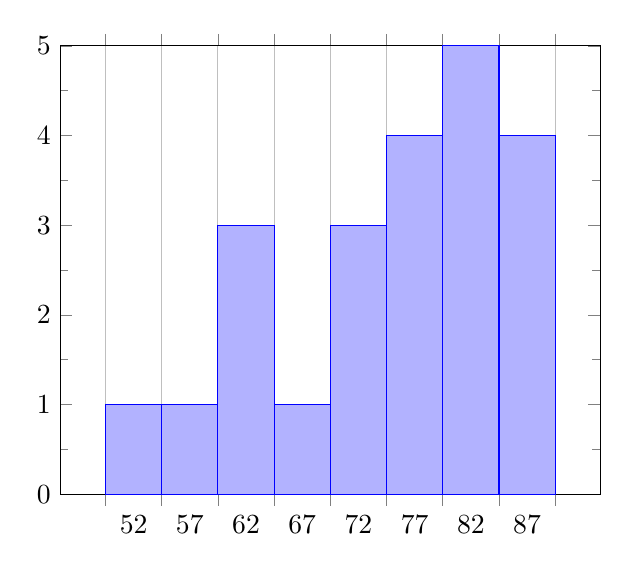
\begin{tikzpicture}
        \begin{axis}[ybar interval, ymax = 5, ymin = 0, minor y tick num = 1]
            \addplot coordinates { (52, 1) (57, 1) (62, 3) (67, 1) (72, 3) (77, 4) (82, 5) (87, 4) (92, 3) };
        \end{axis}
    \end{tikzpicture}
}

\subsubsection{Cumulative Distribution, Percentiles \& Percentile Ranks}
\sectiondefinition{Cumulative Distribution}
{
    A cumulative distribution indicates the percentage of scores that are \underline{less than or equal} to each value.
}
\sectiondefinition{Percentile Rank}
{
    The \underline{percentage} of the distribution that is below a specific score (0\% - 100\%) (y-axis)
    \newline 
    \textit{Ex:} "The percentile rank of a score of 85 is 75\%."
}
\sectiondefinition{Percentile}
{
    This is the score that exceeds a given percentage of the distribution. (x-axis)
    \newline
    \textit{Ex:} "The 40th percentile is an exam score of 75."
}

\subsubsection{Stem-and-leaf Displays}
These are typically excellent for visualizing a distribution. They're used more for 
\textit{exploring data} than for presenting to an audience. 

\section{Describing Data Using Numbers}
\subsubsection{Measures of Center}
\begin{enumerate}
    \item Mode - the most frequent value. Think of a bell curve, where the tip is the mean. Often times a single bell curve is "unimodal". 
    However, they can also be "bimodal".
    \item Median - the score in the middle of the distribution. (the 50th percentile.) 
    To find the location of the median in an ordered array, use the formula : (N + 1)/2. \textit{NOTE: That this is \underline{NOT} how you FIND the median.}
    \item Mean - $\bar{x}$ = $\frac{\sum x}{N}$. The mean is the balance point of the distribution.
\end{enumerate}

\noindent Sample mean: $\bar{x}$ = $\frac{\sum x}{n}$ (This is a \underline{statistic}, since it describes a sample.) 
\newline
Population Mean: $\mu$ = $\frac{\sum x}{N}$ (This is a \underline{parameter}, since it describes a population.)

\sectionexample{\underline{Number of sexual partners}}
{
    
    \textbf{\underline{Bottom line:} The mean can be misleading when there are extreme scores. To really understand your data, look at \underline{all three} measures of center.}
}

\subsubsection{Key Features of Means}
% try to use multicol here instead 
\begin{itemize}
    \item $\sum(x - \bar{x})$ always = 0
    \begin{itemize}
        \item 3
        \item 4
        \item 5
        \item 6
        \item 7
    \end{itemize} 
    The mean of this data set is 5. ($\bar{x}$ = 5)
    \begin{itemize}
        \item -2
        \item -1
        \item 0
        \item 1
        \item 2
    \end{itemize}
    These are the "Deviation scores"; $\sum(x - \bar{x})$ = 0.00

    \item The sum of the squared deviations $\sum(x - \bar{x})^2$ is minimized by the mean.
    \begin{itemize}
        \item 3
        \item 4
        \item 5
        \item 6
        \item 7
    \end{itemize}
    The mean is 5.00. ($\bar{x}$ = 5.00)
    \begin{itemize}
        \item -2
        \item -1
        \item 0
        \item 1
        \item 2
    \end{itemize}
    The sum of the deviation score is 0.00. ($\sum(x - \bar{x})$ = 0.00)
    \begin{itemize}
        \item 4
        \item 1
        \item 0
        \item 1
        \item 4
    \end{itemize}
    The sum of the squared deviations is 10.00. ($\sum(x - \bar{x})^2$ = 10.00)
    \item Try another value where $\bar{x}$ = 4
    \begin{itemize}
        \item 1
        \item 0
        \item 1
        \item 4
        \item 9
    \end{itemize}
    The sum of the squared deviations is 15.00. ($\sum(x - \bar{x})^2$ = 15.00)
\end{itemize}

Only the \underline{mean} keeps the seesaw balanced! That's because $\sum(x - \bar{x})$ = 0.00. 
For skewed distributions, the \underline{median} is most useful.

\section{Measures of Spread}

\subsection{Three Most Common Measures of Spread}
These are going from least to most sophisticated ways of measuring spread.
\begin{itemize}
    \item Range = Largest - Smallest
    \item Variance = $\frac{\sum(x - \bar{x})^2}{N}$. \textit{Ex: }
    \begin{multicols}{3}
        The following are X
        \begin{itemize}
            \item 3
            \item 4
            \item 5
            \item 6
            \item 7
        \end{itemize}
        $\bar{x}$ = 5.00

        \columnbreak
        The following are X - $\bar{x}$
        \begin{itemize}
            \item -2
            \item -1
            \item 0
            \item 1
            \item 2
        \end{itemize}
        $\sum(X - \bar{x})$ = 0.00

        \columnbreak
        The following is $(X - \bar{x})^2$
        \begin{itemize}
            \item 4
            \item 1
            \item 0
            \item 1
            \item 4
        \end{itemize}
        $\sum(X - \bar{x})^2$ = 10.00 \textit{Note: This is also called sum of the squared deviations, or "sum of squares" or "SS"}
    \end{multicols}
    In the end, the variance is 2.00.
    \item Standard Deviation = $\sqrt{Variance}$. \textit{Ex: } $\sqrt{2.00}$ = 1.41. \textbf{Memorize this for the exam.}
\end{itemize}

\noindent Standard Deviation = $S_x = \sqrt{\frac{\sum(x - \bar{x})^2}{N}}$
\newline
Population Standard Deviation = $\sigma_x = \sqrt{\frac{\sum(x - \mu)^2}{N}}$
\newline 
Estimated Population Standard Deviation = $s_x = \sqrt{\frac{\sum(x - \bar{x})^2}{n-1}}$
\newline\newline
The first two are used when \underline{describing} data. The third is used when making \underline{inferences}. All three of these are "center-based" measures of spread. 

\sectionexample{Number Of times Rated}
{
    \begin{multicols}{3}
        The following is X
        \begin{itemize}
            \item 0
            \item 5
            \item 3
            \item 0
            \item 2
            \item 4
            \item 5
            \item 6
        \end{itemize}
        $\sum x$ = 25. $\bar{x}$ = 3.12.

        \columnbreak
        The following is X - $\bar{x}$
        \begin{itemize}
            \item -3.12
            \item 1.87
            \item -.13
            \item -3.12
            \item -1.13
            \item .87
            \item 1.87
            \item 2.87
        \end{itemize}
        $\sum(X - \bar{x})$ = 0.00

        \columnbreak
        The following is $(X - \bar{x})^2$
        \begin{itemize}
            \item 9.50
            \item 3.50
            \item .02
            \item 9.80
            \item 1.28
            \item .76
            \item 3.50
            \item 8.24
        \end{itemize}
        $\sum(X - \bar{x})^2$ = 36.88
    \end{multicols}
    Finally, using the standard deviation formula of $S_x = \sqrt{\frac{\sum(x - \bar{x})^2}{N}}$, we get a standard deviation of 2.15
}

\section{Know your Stat Calculator!}
\begin{itemize}
    \item Be sure you are familiar with its stat functions.
    \begin{itemize}
        \item Esp. standard deviation and variance
        \item (N) or (N-1) on denominator?
        \item \underline{Easy check:}
        \begin{enumerate}
            \item Enter these values: {1, 2, 3}
            \item std. dev = .82 when using N in denominator (descriptive)
            \item std. dev = 1.00 when using N-1 in denominator (inferential)
        \end{enumerate}
    \end{itemize}
    \item Got a TI-30Xa? Then watch the video that was posted by Dr. Tyrell in Canvas.
\end{itemize}

\section{Complete Descriptions of Data}
\begin{itemize}
    \item To \underline{completely} describe a variable, describe its:
    \begin{enumerate}
        \item Center 
        \begin{itemize}
            \item Mean, median, mode
        \end{itemize}
        \item Spread
        \begin{itemize}
            \item Range, standard deviation, variance
        \end{itemize}
        \item Form 
    \end{enumerate}
\end{itemize}
We've talked about the first two but what about \underline{form}?

\subsection{Measures of Form}
\begin{enumerate}
    \item Modality - The number of peaks in a distribution. \textit{Ex: Unimodal or bimodal.}
    \item Skewness - The degree to which a distribution is asymmmetrical. \textit{Ex: Positively (right \& (mean < median < mode)) or negatively (left \& (mode < median < mean)) skewed.} 
    \item Kurtosis - The degree to which a distrbution is peaked or flat. \textit{Ex: Leptokurtic (peaked) or platykurtic (flat).}
\end{enumerate}
And these are great, however the best way to see the form of a variable is to use a histogram.

\section{Transformations}

\underline{Effect of transformations on the CENTER:}
\begin{enumerate}
    \item Adding or subtracting a constant from all data points has same effect on center. 
    \item Multiplying or dividing all data points by a constant has same effect on center.
\end{enumerate}
\underline{Effect of transformations on the SPREAD:}
\begin{enumerate}
    \item Adding or subtracting a constant has NO effect on spread.
    \item Multiplying or dividing by a constant has same effect on measures of spread (\underline{except the variance!})
    \item Multiplying or dividing a constant multiplies or divides the variance by the \underline{square} of the constant.
\end{enumerate}
\sectionexample{Example of transformation}
{
    \begin{multicols}{3}
        The following is X
        \begin{itemize}
            \item 1
            \item 10
            \item 15
        \end{itemize}
        \begin{itemize}
            \item 8.67 (Mean)
            \item 5.79 (Standard Deviation)
            \item 33.56 (Variance)
        \end{itemize}
        \columnbreak
        plus 10
        \columnbreak
        The following is X + 10
        \begin{itemize}
            \item 11
            \item 20
            \item 25
        \end{itemize}
        \begin{itemize}
            \item 18.67 (Mean)
            \item 5.79 (Standard Deviation [unchanged])
            \item 33.56 (Variance [unchanged])
        \end{itemize}
    \end{multicols}
}
\sectionexample{Example of transformation}
{
    \begin{multicols}{3}
        The following is X
        \begin{itemize}
            \item 1
            \item 10
            \item 15
        \end{itemize}
        \begin{itemize}
            \item 8.67 (Mean)
            \item 5.79 (Standard Deviation)
            \item 33.56 (Variance)
        \end{itemize}
        \columnbreak
        times 10
        \columnbreak
        The following is X * 10
        \begin{itemize}
            \item 10
            \item 100
            \item 150
        \end{itemize}
        \begin{itemize}
            \item 86.67 (Mean [multiplied by 10])
            \item 57.93 (Standard Deviation [multiplied by 10])
            \item 3356.00 (Variance [multiplied by 100])
        \end{itemize}
    \end{multicols}
}

\chapter{Exam 2}

\section{z-scores and normal curves}
\sectionexample{z-scores}
{
    \begin{multicols}{3}
        The following are X
        \begin{itemize}
            \item 17
            \item 1824
            \item 27
            \item 32
        \end{itemize}
        The mean: 23.60. 
        Standard Deviation: 5.61
        \columnbreak
        The following is X - $\bar{x}$
        \begin{itemize}
            \item -6.6
            \item -5.6
            \item .4
            \item 3.4
            \item 8.4
        \end{itemize}
        Mean: 0.00 
        Standard Deviaton: 5.61 
        \columnbreak
        The following is $\frac{X - \bar{x}}{s}$
        \begin{itemize}
            \item -1.18
            \item -1.00
            \item .07
            \item .61
            \item 1.49
        \end{itemize}
        These are the z-scores. 
        Mean: 0.00
        Standard Deviation: 1.00
    \end{multicols}
}

\subsection{5 Characteristics of the Normal Curve}
\begin{enumerate}
    \item Unimodal
    \item Symmetrical
    \item Bell-shaped
    \item Asymptotic
    \item The "66-95-99.7" rule (Emperical rule)
\end{enumerate}

\subsection{3 Characteristics of z-scores}
\begin{enumerate}
    \item Mean of all z scores always = 0
    \item Std dev of all z scors always = 1
    \item z distribution always has same shape as original distribution
\end{enumerate}

\subsection{3 advantages of z-scores}
\begin{itemize}
    \item z-scores do not ignore the distance between scores (percentiles do)
    \item z-scores allow you to compare scores from different distributions
    \item If you have (or assume) a normal distribution, z-scores allow you to calculate the proportion of scores that fal between \underline{any} given range of scores.
\end{itemize}

\noindent\underline{"Standard Normal Curve"} A normal distribution with a mean of 0 and a standard deviation of 1. Allows us to translate \underline{any} normal distribution into the \underline{standard normal curve}. $Z = \frac{X - \bar{x}}{s_x}$
\newline\newline
\noindent On page 422 there is a table C.1 that shows the proportion of scores that fall between any given range of z-scores. 

\subsection{Z-score problems}
\sectionexample{What percentage of IQ scores are > 100?}
{
Where the std is 15 and the mean is 100. \newline
IQ: 70, 85, 100, 115, 130 \newline
Z: -2, -1, 0, 1, 2 \newline

$Z = \frac{X - \bar{x}}{s}$ = $\frac{100 - 100}{15}$ = 0.00. \newline
The answer to this is 50\%.
}

\sectionexample{What percentage of IQ scores are greater than 105?}
{
Where the std is 15 and the mean is 100. \newline
IQ: 70, 85, 100, 115, 130 \newline
Z: -2, -1, 0, 1, 2 \newline 

$Z = \frac{X - \bar{x}}{s}$ = $\frac{105 - 100}{15}$ = 0.33. \newline
The answer would be 37.07\%.
}


\sectionexample{What proportion of IQ scores are less than 90?}
{
Where the std is 15 and the mean is 100. \newline
IQ: 70, 85, 100, 115, 130 \newline 
Z: -2, -1, 0, 1, 2 \newline

We want to look at the IQ scores of 90 and less. 
$Z = \frac{X - \bar{x}}{s}$ = $\frac{90 - 100}{15}$ = -0.67. \newline
The answer would be .2514.
}

\sectionexample{What percentage of IQ scores are > 87}
{
Where the std is 15 and the mean is 100. \newline
IQ: 70, 85, 100, 115, 130  \newline
Z: -2, -1, 0, 1, 2 \newline

We want to look at the IQ scores of 87 and above.
$Z = \frac{X - \bar{x}}{s}$ = $\frac{87 - 100}{15}$ = -0.87. \newline
The answer would be .3078 + .5000 = .8078 which is 80.78\%.
}

\sectionexample{What proportion of IQs are between 112 and 130?}
{
Where the std is 15 and the mean is 100. \newline
IQ: 70, 85, 100, 115, 130 \newline
Z: -2, -1, 0, 1, 2 \newline

We want to look at the IQ scores between 112 and 130. \newline
$Z = \frac{X - \bar{x}}{s}$ = $\frac{130 - 100}{15}$ = 2.00. \newline
$Z = \frac{X - \bar{x}}{s}$ = $\frac{112 - 100}{15}$ = 0.80. \newline

From the table, we can see that 2.00 = .4772 and .8000 = .2881 We then want to subtract the biggest number and the smallest to get our proportion. \newline
.4772 - .2881 = .1891.
}

\sectionexample{What is the percentage of IQ scores between 0.5 and 1.5 standard deviations above the mean?}
{
Where the std is 15 and the mean is 100. \newline
IQ: 70, 85, 100, 115, 130 \newline
Z: -2, -1, 0, 1, 2 \newline

We want to look at the IQ scores between 0.5 and 1.5 standard deviations above the mean. \newline
1.5 = .4332. \newline
.5 = .1915. \newline
.4332 - .1915 = .2417 which is 25.17\% \newline 
}

\sectionexample{What z-score corresponds to the $40^{th}$ percentile?}
{
Where the std is 15 and the mean is 100. \newline
IQ: 70, 85, 100, 115, 130 \newline
Z: -2, -1, 0, 1, 2 \newline

We want to look at the bottom 40\% of the data from the upper 60\%. \newline
$Z = \frac{X - \bar{x}}{s}$ = $\frac{X - 100}{15}$ = -0.255. \newline
}

\sectionexample{What IQ score corresponds to the 25th percentile?}
{
Where the std is 15 and the mean is 100. \newline
IQ: 70, 85, 100, 115, 130 \newline
Z: -2, -1, 0, 1, 2 \newline

We want to look at the bottom 25\% of the data from the upper 75\%. \newline
$Z = \frac{X - \bar{x}}{s}$ = $\frac{X - 100}{15}$ = -0.675. \newline
Split two numbers from the textbook column in half to get this Z score. \newline
Now, to find the IQ score we do the following: \newline

$X = \bar{x} + Zs$ = $100 + (-0.675)(15)$ = 89.875. \newline
}

\sectionexample{What 2 z-scores surround the central 95\% of a normal distribution?}
{
Where the std is 15 and the mean is 100. \newline
IQ: 70, 85, 100, 115, 130 \newline
Z: -2, -1, 0, 1, 2 \newline

We want to look at the central 95\% of the data. \newline
Split the 95\% in half to get 47.5\% on each side. \newline
From the table, we can see that 1.96 = .4750. \newline
The two z-scores are -1.96 and 1.96. \newline
}

\section{Correlations}
\subsection{Scatterplots}
\textit{Note:} The x-axis is called the abscissa and the y-axis is called the ordinate. \newline 
\begin{itemize}
    \item Strong \underline{positive} relationship. When X goes up, Y goes up.
    \item Strong \underline{negative} relationship. When X goes up, Y goes down.
\end{itemize}

\subsection{Correlation Coefficient}
\begin{itemize}
    \item A single number that describes the strength of the linear relationship betwene two variables. 
    \item Value is always between -1 and +1. A perfect negative correlation is -1 and a perfect positive correlation is +1. A 0 means no correlation.
\end{itemize}

There are two different kinds of correlation coefficients. 
\begin{itemize}
    \item Pearson's product-moment correlation coefficient (r)
    \item Spearman's rank-order correlation coefficient ($r_s$)
\end{itemize}

\subsection{Calculating Pearson's R}
\sectionexample{Example 1}
{
    \begin{multicols}{5}
        X 
        \begin{itemize}
            \item 6
            \item 9
            \item 4
            \item 2
            \item 4
        \end{itemize}
        \columnbreak
        Y
        \begin{itemize}
            \item 7
            \item 4
            \item 6
            \item 10
            \item 3
        \end{itemize}
        \columnbreak
        X - $\bar{x}$
        \begin{itemize}
            \item 1
            \item 4
            \item -1
            \item -3
            \item -1
        \end{itemize}
        \columnbreak
        Y - $\bar{y}$
        \begin{itemize}
            \item -3
            \item 4
            \item 1
            \item -2
            \item 0
        \end{itemize}
        \columnbreak
        $(X - \bar{x})(Y - \bar{y})$
        \begin{itemize}
            \item -3
            \item 16
            \item -1
            \item 6
            \item 0
        \end{itemize}
        $\sum(X - \bar{x})(Y - \bar{y})$ = 18.00

    \end{multicols}
    Mean of X = 5.00. \newline
    Mean of Y = 3.00. \newline
    S of X = 2.37. \newline
    S of Y = 2.45. \newline

    \underline{Pearson's r} = $\frac{cov(x, 4)}{s_x s_y}$. \newline 
    Where cov(x, y) = $\frac{\sum(X - \bar{x})(Y - \bar{y})}{N}$ = $\frac{18}{5} = 3.6$ \newline
    \textit{Note: N is the number of pairs of observations} \newline
    \textit{Note: Covariance and correlation are always the same sign.} \newline 
    \textit{Note: Covariance is big when variance is big.} \newline\newline 

    $r = \frac{cov(x, y)}{s_x s_y} = \frac{3.6}{2.37 * 2.45}$ = +0.62. \newline
}

\sectionexample{Example 2}
{
    Let's try a new but same equation. $r = \frac{cov(x, y)}{s_x s_y} = \frac{\sum(z_x z_y)}{N}$. \newline
    Using the same previous data, we can find Z. \newline 
    \begin{multicols}{3}
        Z of X
        \begin{itemize}
            \item .42
            \item 1.69
            \item -.42
            \item -1.27
            \item -.42
        \end{itemize}
        \columnbreak
        Z of Y
        \begin{itemize}
            \item -1.22
            \item 1.63
            \item .41
            \item -0.82
            \item 0
        \end{itemize}
        \columnbreak
        Z of X * Z of Y
        \begin{itemize}
            \item -.512
            \item 2.755
            \item -.172
            \item 1.041
            \item 0
        \end{itemize}
        $\sum(Z_x Z_y)$ = 3.112
    \end{multicols}
    $r = \frac{cov(x, y)}{s_x s_y} = \frac{3.112}{5} = 0.62$. \newline
    \textit{Note: Pearson's r is the "average correspondance between pairs of z-scores".}
}

\subsection{Three ways to calculate Pearson's r}
\subsection{Pearson's vs Spearman's}
\begin{itemize}
    \item Pearson's r only applies when both variables are either \underline{interval} or \underline{ratio} measurement scales. \textit{Note: It's based on difference scores!}
    \item If either variable (or both) is \underline{ordinal}, use Spearman's.
    \item There are 2 approaches to calculating Spearman's. 
    \begin{enumerate}
        \item Use the textbook's formula.
        \item Use the "Tyrrell method"
    \end{enumerate}
\end{itemize}

\subsubsection{The Tyrrell Method}
\underline{The Tyrrell approach to calculating Spearman's r}
\begin{enumerate}
    \item Convert both variables to ranks. 
    \item Apply Pearson's formulas to the ranks. 
\end{enumerate}

\section{Linear Regression}
Remember: Correlations describe the strength of the linear relationship between two variables. 
\begin{itemize}
    \item But once we've \underline{described} it, can we use it to make predictions?
    \item \textit{Ex:} Predicting weight\dots
\end{itemize}
Regression: "Model" the relationship and use the model to make predictions. 
\begin{itemize}
    \item Our model will be based on simple linear algebra: $Y = a + bX$
    \item Where Y is the predicted value of the dependent variable, X is the value of the independent variable, a is the Y-intercept, and b is the slope of the line.
    \item If the slope is positive, the relationship is positive. If the slope is negative, the relationship is negative.
    \item Our model minimizes the sum of the squared residuals. 
    \item That is, the goal of regression is to build a model that minimizes this: $\sum (Y - Y')^2$.
    \item Therefore, regression models are often called "least squares" models.
\end{itemize}

\newpage
\sectionexample{Example 1}
{
    Using the same X, Y numbers from example 1 of Calculating Pearson's R: \newline\newline
    $B = \frac{N\sum XY-(\sum X)(\sum Y)}{N\sum X^2 - (\sum X)^2}$. \newline

    \begin{multicols}{2}
        $X^2$
        \begin{itemize}
            \item 36
            \item 81
            \item 16
            \item 4
            \item 16
        \end{itemize}   
        \columnbreak
        $XY$
        \begin{itemize}
            \item 18
            \item 90
            \item 28
            \item 8
            \item 24
        \end{itemize}
    \end{multicols}

    $b = \frac{5(168) - (25)(168)}{5(153) - (25)^2}$ = $\frac{840 - 750}{765 - 625}$ = .64. \newline\newline
    Y = 0.64X \newline
    
    Or, $b = r(S_y/S_x)$ = 0.62(2.45/2.37) = 0.64. \newline\newline
    Y = 0.64X \newline

    $a = \bar{y} - b\bar{x}$ = 6.0 = (.64)(5.0) = 2.80 \newline

    Now we have Y = 2.80 + 0.64X. \newline
    \begin{multicols}{3}
        $Y'$
        \begin{itemize}
            \item 6.64
            \item 8.56
            \item 5.36
            \item 4.08
            \item 5.36
        \end{itemize}
        \columnbreak
        $Y - Y'$
        \begin{itemize}
            \item -3.64
            \item 1.44
            \item 1.64
            \item -.08
            \item .64
        \end{itemize}
        \columnbreak
        $(Y - Y')^2$
        \begin{itemize}
            \item 13.25
            \item 2.07
            \item 2.69
            \item .01
            \item .41
        \end{itemize}
        $\sum(Y - Y')^2$ = 18.43
    \end{multicols}

    $S_y' = \sqrt{\frac{\sum(Y - Y')^2}{N}}$ = $\frac{\sqrt{18.43}}{5}$ = 1.92 \newline
}

Residual = prediction error = observed - predicted. \newline\newline 

\underline{Think of the regression line as:}
\begin{itemize}
    \item The regression model.
    \item All predicted values connected together.
    \item The 2-dimensional \underline{center} of the data.
\end{itemize}
\underline{Think of the standard devation error of the estimate $S_y$ as:}
\begin{itemize}
    \item A 2-dimensional measure of \underline{spread}.
    \item "average error" of model
\end{itemize}
\underline{Strong correlations give:}
\begin{itemize}
    \item Strong models
    \item Small residuals
    \item Small $S_(y')$
\end{itemize}
\underline{Weak correlations give:}
\begin{itemize}
    \item Weak models
    \item Big residuals
    \item Big $S_(y')$
\end{itemize}

\sectionexample{Regression Example: Handwriting \& Personality}
{
    Specifically: Can extraversion be predicted by loop width? \newline 
    Where extraversion is a personality characteristic and width (in mm) of the loops in the letters a, p, and d. \newline
}

\subsubsection{\underline{"Proportion of variance accounted for"}}

Using $\bar{Y}$ to predict Y scores results in lots of error. However, using the known relationship to predict Y scores results in less error. But \underline{how much} less? \newline

\subsubsection{\underline{$r^2$ measures "predictable variability"}}

(Remember: r is the correlation coefficient.)\newline 
$r^2$ tells us \underline{the proportion of variance in Y that can be predicted in X}. \newline

\begin{multicols}{3}
    \noindent If r = .20, $r^2$ = .04. X predicts 4\% of the variance of Y.
    \columnbreak

    If r = .50, $r^2$ = .25. X predicts 25\% of the variance of Y. 
    \columnbreak
    
    If r = .90, $r^2$ = .81. X predicts 81\% of the variance of Y.
\end{multicols}
\noindent $r^2$ is the best way to evaluate the scientific \underline{importance} of a relationship. 

\section{Probability}

\subsection{Three probability rules}
\begin{enumerate}
    \item When outcomes are equally ikely, the probability of an event is: p = $\frac{number of possibilities of that event}{total number of possibilities}$
    \item This is called the "additive rule". The probability of \underline{either} of two mutually eclusive events occurring is the \underline{sum} of their separate probabilities.
    \item This is called the "multiplicative rule". The probability of two independent events \underline{both} occuring is the \underline{product} of their separate probabilities.
\end{enumerate}

\underline{Notice that:} Using the additive rule $\uparrow$ probability, but using the multiplicative rule $\downarrow$ probability. Apply this to the simple lottery\dots

\sectionexample{Powerball Math}
{
    \begin{itemize}
        \item Odds of winning the big jackpot:
        \begin{itemize}
            \item 1 in 292,201,338
        \end{itemize}
        \item \underline{If you buy 25 tickets/week (@ \$2):}
        \begin{itemize}
            \item You can expect to win once every 225,000 years
        \end{itemize}
        \item A lottery is a "zero-sum game."
    \end{itemize}
}

\sectiondefinition{Bernoulli's Theorem "The law of large numbers"}
{
    Predicts that as N gets larger the frequency of an event will approach (p*N). \newline 

    In other words\dots As N increases, we can expect the frequnecies to be closer and closer to the predicted frequencies.
}

\section{Sampling Distribution}

\sectionexample{Example 1}
{
    The population: \newline 
    Body weights of all 30 students in a class. \newline
    $\mu = 139.9$ \newline
    $N = 30$ \newline

    Let's pick a few samples, each of size n = 2\dots (n is sample size, N is population size) \newline\newline 
    \underline{Every possible sample mean:} Sample means will fluctuate, even though population means do not. \newline\newline 
}

\sectiondefinition{Sampling Distribution}
{
    A distribution of the probabilities of \underline{all possible values} of a statistic. \textit{These are important because they tell us how much sample-to-sample variability we should expect in our statistic.}

    This is represented by the "sampling distribution of every possible sample mean." \newline 
    $\mu_{\bar{x}} = $ "Mean of all the x bar" \newline
    $\sigma_{\bar{x}} = $ "Standard deviation (error) of the x bars" \newline
}

\subsection{Standard Error of the Mean}
\begin{itemize}
    \item The S.E.M is the standard deviation of a sampling distribution.
    \item "How spread out are the sample means?" or "How much error can you expect to be in your sample mean?"
    \item The S.E.M depends on only 2 factors: 
    \begin{enumerate}
        \item As $\sigma$ increases, the S.E.M increases.
        \item As n increases, the S.E.M decreases.
    \end{enumerate}
    \item Formula for S.E.M: $\sigma_{\bar{x}} = \frac{\sigma}{\sqrt{N}}$ {\textit{Note: $\sigma$ is the standard deviation of the population.} \textbf{THIS IS ANOTHER FORMULA TO MEMORIZE}}
\end{itemize}

\subsubsection{How can we fully describe a sampling distribution?} 
\begin{itemize}
    \item We'll \underline{rarely} take every possible sample from a population. 
    \begin{itemize}
        \item Normally, we only take one!
    \end{itemize}
    \item So, we need a system of shortcuts tto allow us to describe a sampling distribution. 
\end{itemize}

\subsection{Central Limit Theorem}
\begin{itemize}
    \item Center: Mean of sampling distribution = mean of the population. $\mu_{\bar{x}} = \mu$
    \item Spread: Standard deviation of sampling distribution = S.E.M.: $\sigma_{\bar{x}} = \frac{\sigma}{\sqrt{N}}$
    \item Form: "As n increases, sampling distribution becomes more normal." Also, if the population is normal, then the S.D is as well (regardless of n).
\end{itemize}

\sectionexample{Central Limit Theorem In Action}
{
    \underline{Extreme Example:} Start with a population that's \underline{not} normally distributed. \textit{Ex: all numbers from 0 - 100, evenly distributed.} \newline 
    $\mu = 50$ \newline
    $\sigma = 28.9$ \newline
    Even with a small N (just 4), sampling distribution looks \underline{somewhat} normal. \newline
    $\mu_{\bar{x}} = 50$ \newline
    $\sigma_{\bar{x}} = \frac{\sigma}{\sqrt{N}} = \frac{28.9}{\sqrt{4}} = 14.43$ \newline
    But now, with a larger N (30), sampling distribution looks \underline{very} normal. \newline
    $\mu_{\bar{x}} = 50$ \newline
    $\sigma_{\bar{x}} = \frac{\sigma}{\sqrt{N}} = \frac{28.9}{\sqrt{30}} = 5.27$ \newline
    Remember: C.L.T says that as N increases the sampling distribution becomes normal and the S.E.M shrinks. \newline\newline

    What these look like visually, the smaller the N, the graph tends to look more wider, but as N increases, the graph tends to look more normal and skinnier.
}

\subsection{\underline{Using} Sampling Distributions}
What if we take a sample from this population and our $\bar{x}$ is 160? Maybe our mean is from a \underline{different} population?
How far from 139 can our $\bar{x}$ get before we decide something weird is going on? In order to answer questions like this we will have to rely on three tools. \newline 
\begin{enumerate}
    \item Probability (three rules and a low)
    \item Knowledge of sampling distributions
    \item Logic of \underline{hypothesis testing}
\end{enumerate}

\section{Hypothesis Testing}

\sectionexample{Example of Hypothesis Testing}
{
    Your particular interest is in behavior problems in stressed children. Mean beahvior problems score of general population is 50. 
    We have access to five children whose parents are newly divorced. Their mean is 53. \newline\newline 
    Can we conclude that stressed children exhibit an increased number of behavior problems? 
    Is the +3 difference due to a \underline{real effect} of stress or is it due to \underline{sampling error}? \newline\newline 

    The distribution of all possible sample means of behavior problems, each based on n = 5 scores. This shows as a normal distribution of a simpling distribution on a histogram. \newline\newline 

    What's the probability of getting a smple mean of 53 if you're sampling from a population with a mean of 50? \newline\newline 

    The first kind of hypothesis testnig we'll do is the easist\dots: The z-test.
}

When using the z-test, we can take interest in answering the following question. "Does this particlar sample come from a poulation with a mean of [insert hypothesized value of $\mu$ here]?" \newline

\subsection{Seven steps involved in hypothesis testing}

\begin{enumerate}
    \item Define the null hypothesis, $H_0$.
    \begin{itemize}
        \item Statement of the parameter value that we want to test. \textit{Note: Must state a specific parameter and give it a value.}
        \item Example: $H_0: \mu = 50$
        \item Usually asserts that a more interesting hypothesis is wrong. 
        \item $H_0$ is the hypothesis that we actually test. 
    \end{itemize}
    \item Specify the alternative hypothesis, $H_a$ (also called the research hypothesis).
    \begin{itemize}
        \item Logical opposite to the null hypothesis.
        \item $H_a$ and $H_0$ must be mutually exclusive and exhaustive.
        \item $H_a$ is usually the hypothesis we hope to support. 
        \item Example: $H_a: \mu \neq 50$
    \end{itemize}
    \item Construct the sampling distribution under the assumption that the null hypothesis is true.
    \begin{itemize}
        \item What would be the \underline{center, spread, and form} of the sampling distribution if $H_0$ were true?
        \begin{itemize}
            \item Center usually specified by $H_0$.
            \item Spread = standard error of the mean. 
            \item Form: Is it normal? 
        \end{itemize}
    \end{itemize}
    \item Collect the Data
    \item Compare the sample statistic to the value in $H_0$.
    \item \underline{Find the probability} of exceeding the observed statistic's value.
    \item Make the inference. 
    \begin{itemize}
        \item Decide which decision to make\dots only two possibilities. 
        \item Either \textbf{reject $H_0$} (if it is \underline{unlikely} to be true)
        \item or \textbf{fail to reject $H_0$} (if it is \underline{likely} to be true)
    \end{itemize}
\end{enumerate}
\begin{itemize}
    \item Remember, this logic is indirect:
    \begin{itemize}
        \item We're testing the hypothesis that we hope is wrong ($H_0$).
        \item If we reject $H_0$, we've found indirect evidence to support $H_a$.
    \end{itemize}
\end{itemize}

\subsubsection{New form of Z}

$Z_{calc} = \frac{\bar{X} - \mu}{\sigma_{\bar{x}}} \leftarrow$ "How many standard error of the means is my sample mean from the $H_a$ value?" \newline\newline 

If $\abs{Z_{calc}} > Z_{critical}$, then reject $H_0$. \newline
Fail to rject because (finish this its in iphone photos)


\subsection{Errors in Making Inferences} 

\begin{table}
    \centering
    \begin{tabular}{|c|c|c|}
        \hline
        & \textbf{True $H_0$} & \textbf{False $H_0$} \\
        \hline
        \textbf{Fail to reject $H_0$} & Correct decision $p = 1 - \alpha$ & Type II error (keeping a false $H_0$) $p = \beta$\\
        \hline
        \textbf{Reject $H_0$} & Type I error (rejecting a true $H_0$) $p = \alpha$ & Correct decision $p = 1 - \beta$ "power" \\
        \hline
    \end{tabular}
    \caption{Table of our inference and actual state of nature}
\end{table}

\subsubsection{Statistical Power}
\begin{itemize}
    \item The probability of correctly rejecting a false null hypothesis. 
    \item $p = 1 - \beta$
\end{itemize}

\subsubsection{Power is influenced by four things:}
\begin{enumerate}
    \item $\mu$ (father from $H_O$, the more power)
    \item $\sigma$ (smaller the sigma the more power) 
    \item $\alpha$ (bigger the alpha the more power)
    \item N (more data the more power) 
    \item \textit{Note: Number 3 and 4 are within your control.}
\end{enumerate}

\subsection{Why is it good to get more data?}
\begin{itemize}
    \item Because as we get $\uparrow N$, we get \underline{more power}
    \item But how? 
    \item $\uparrow N \rightarrow \downarrow \sigma_{\bar{x}} \rightarrow \uparrow Z_{calc} \rightarrow$ easier to reject a false $H_O$ (this is what "more power" means).
\end{itemize}

\chapter{Exam 3}

\section{Testing a Sample Mean when $\alpha$ is Unknown}
\textit{Note: What we are not covering - 1. Confidence intervals (p 246 - 248), 2. Testing correlations. (p 249 - 255)}

\sectiondefinition{William Gosset's Contribution}
{ % make this into columns soon
    Z-Test = $z_{calc} = \frac{\bar{X} - \mu}{\sigma_{\bar{X}}}$ \newline
    where: \newline
    $\sigma_{\bar{X}} = \frac{\sigma}{\sqrt{N}}$ \newline

    "Student's 1-sample t Test" = $t_{calc} = \frac{\bar{x} - \mu}{s_{\bar{X}}}$ \newline
    where: \newline
    $s_{\bar{x}} = \frac{s}{\sqrt{N}}$ \newline
    and: \newline 
    $s = \sqrt{\frac{\sum(X - \bar{X})^2}{N - 1}}$ \newline
    and: \newline
    \begin{itemize}
        \item "df" = "degrees of freedom"
        \item $t_{crit}$
        \item 
    \end{itemize}
}

\sectionexample{Example of a 1-sample T-Test}
{
    Q: You're told that the national average for \# of hours / week worked by business consultants is 52. Are you employees significantly different? Use $\alpha = .05$. \newline

    $H_0: \mu = 52$ \newline
    $H_a: \mu \neq 52$ \newline

    We know: \newline
    $\alpha = .05$ \newline
    $N = 16$ \newline
    $\bar{X} = 59$ hr/week \newline
    $s = 7.15$ hr/week \newline 
    Population is normal. \newline

    Describe the sampling distribution assuming $H_0$ is true: \newline 
    \begin{enumerate}
        \item $\mu_{\bar{X}} = 52$ 
        \item $\sigma_{\bar{X}} = \frac{\sigma}{\sqrt{N}} = \frac{7.15}{\sqrt{16}} = 1.79$ 
        \item Sampling Distribution is normal. 
        \begin{itemize}
            \item $df = N - 1 = 16 -1 = 15$
            \item $t_{crit} = \pm 2.131$
            \item $t_{calc} = \frac{59 - 52}{1.79} = 3.91$
        \end{itemize}
    \end{enumerate}

    Summarize Statement: 
}

\section{1-tailed vs. 2-tailed tests}

\begin{multicols}{2}
    \begin{itemize}
        \item \underline{Two-tailed Tests} are for testing "non-directional" hypotheses.
        \item "Is $\mu$ significantly different from \dots?"
        \item $H_0: \mu = [some value]$
        \item $H_a: \mu \neq [some value]$
        \item Here, $\alpha$ is split between the 2 tails ($\alpha/2$ in each tail).
    \end{itemize}
    \columnbreak    
    \begin{itemize}
        \item \underline{One-tailed Tests} are for testing "directional" hypotheses.
        \item "Is $\mu$ significantly greater than \dots?"
        \item $H_0: \mu <= [some value]$
        \item $H_a: \mu > [some value]$
        \item Here, $\alpha$ is placed entirely in 1 tail.
        \item 1-tailed tests are more powerful\dots but are riskier, too.
    \end{itemize}
\end{multicols}


\sectionexample{Another Example of 1-sample T-Test}
{
    $\alpha = .05$ \newline
    $N = 21$ \newline 
    $H_0: \mu = 57.4$ \newline 
    $H_a: \mu \neq 57.4$ \newline
    $\bar{X} = 62.4$, $S = 11.00$, $df = 20$, $S_{\bar{X}} = \frac{11}{\sqrt{21}} = 2.41$ \newline
    $t_{calc} = \frac{62.4 - 57.4}{2.41} = 2.07$ \newline
    $t_{crit} = \pm 2.086$ \newline

    1-Tailed Test: \newline 

    $H_0: \mu <= 57.4$ \newline
    $H_a: \mu > 57.4$ \newline
    $\alpha = .05$ \newline
    \textit{Note: $n, \bar{X}, s, and s_{\bar{X}}$ are the same as above.} \newline
    $t_{crit} = 1.725$ \newline
    $t_{calc} = \frac{62.4 - 57.4}{2.41} = 2.07$ \newline 
    Reject the $H_0$ because $t_{calc} > t_{crit}$ \newline\newline 
    \underline{Summary Statement:} \newline 
    \begin{itemize}
        \item Example: The mean stress level of the employees after the CEO's arrest, 62.4, was significantlly greater than 57.4, t(20) = 2.07, p < .05.
        \begin{itemize}
            \item \underline{Note that this statement includes:}
        \end{itemize}
        \item The DV 
        \item The IV 
        \item The value of both means
        \item Whether difference was significant 
        \item Whether a 1- or 2- tailed test was done 
        \item The value of df 
        \item The value of $t_{calc}$
        \item A p-value
    \end{itemize}
}

\subsection{P-values}
\begin{itemize}
    \item p value: the probability of getting your result if the null hypothesis were true. 
    \begin{itemize}
        \item If $H_0$ is rejected then p < $\alpha$. (because it's unlikely)
        \item If $H_0$ is not rejected then p > $\alpha$. (because it's likely)
        \item When you reject $H_0$, end summary statement with "\dots, \underline{p} < .05."
        \item When you fail to reject $H_0$, end with "\dots, \underline{p} > .05."
        \item If an exact p-value is known, give that instead (example, "\dots, \underline{p} = .03.")
    \end{itemize}
\end{itemize}

\section{Experiements with Two Conditions}
\begin{itemize}
    \item Simplest approach to cause-and-effect
    \item The foundation for more complex experiments
\end{itemize}

\begin{itemize}
    \item We need tests to compare 2 sample means.
    \item \underline{\textbf{Two sets of procedures:}}
    \begin{itemize}
        \item 1. Between-subjects expts. (also called "independent samples")
        \item 2. Within-subjects expts. (also called "dependent samples")
    \end{itemize}
    \item We'll assume the two population variances are equal ($\sigma_1^2 = \sigma_2^2$). (i.e., we're assuming "homogenity of variance").
\end{itemize}

\subsubsection{Summary of T-tests:}
\begin{itemize}
    \item One-sample t tests compares Xbar with a hypothesised value (Chapter 11).
    \item Two-sample t tests compare two Xbars (Chapter 12).
    \begin{itemize}
        \item Between-subjects
        \item Within-subjects
    \end{itemize}
    \item For all of the above, general pattern is: $t_{calc} = \frac{observed value - hypothesised value}{standard error}$
\end{itemize}

\section{Between-subjects T-Test Formulas}

\section{Within-subjects T-Test Formulas}

\sectiondefinition{Within Subjects T-Test}
{
    $H_0 : \mu_{diff} = 0$ \newline 
    $H_a : \mu_{diff} \neq 0$ \newline

    \begin{multicols}{4}
        \underline{Subject}
        \begin{itemize}
            \item 1
            \item 2
            \item 3
            \item \dots
            \item N
        \end{itemize}
        Mean: \newline
        S: 
        \columnbreak

        \underline{Score 1}
        \begin{itemize}
            \item 1
            \item 2
            \item 3
            \item \dots
            \item N
        \end{itemize}
        $\bar{X}_{1}$ = $\frac{\sum(X_1)}{N}$ \newline
        $S_{1} = \sqrt{\frac{\sum(X_1)^2}{N - 1}}$ \newline
        \columnbreak

        \underline{Score 2}
        \begin{itemize}
            \item 1
            \item 2
            \item 3
            \item \dots
            \item N
        \end{itemize}
        $\bar{X}_{2}$ = $\frac{\sum(X_2)}{N}$ \newline
        $S_{2} = \sqrt{\frac{\sum(X_2)^2}{N - 1}}$ \newline
        \columnbreak

        \underline{Difference}
        \begin{itemize}
            \item 1
            \item 2
            \item 3
            \item \dots
            \item N
        \end{itemize}
        $\bar{X}_{diff}$ = $\frac{\sum(X_1 - X_2)}{N}$ \newline
        $S_{diff} = \sqrt{\frac{\sum(X_1 - X_2)^2}{N - 1}}$ \newline
    \end{multicols}

    $S_{\bar{X}_{diff}} = \frac{S_{diff}}{\sqrt{N}}$ \newline
    $t_{calc} = \frac{\bar{X}_{diff} - \mu_{diff}}{S_{\bar{X}_{diff}}}$ \newline
}

\sectionexample{Biofeedback \& Headaches}
{
    $H_0: \mu_{diff} = 0$ \newline
    $H_a: \mu_{diff} \neq 0$ \newline
    $\alpha = .05$ \newline
    \begin{multicols}{3}
        \underline{Before Training}
        \begin{itemize}
            \item 17
            \item 13
            \item 6
            \item 5
            \item 5
            \item 10
            \item 8
            \item 6
            \item 7
        \end{itemize}
        $\bar{X}_{1}$ = 8.56 \newline
        $S_{1}$ = 4.10 \newline
        \columnbreak

        \underline{After Training}
        \begin{itemize}
            \item 4
            \item 7
            \item 2
            \item 3
            \item 4
            \item 12
            \item 6
            \item 5
            \item 3
        \end{itemize}
        $\bar{X}_{2}$ = 5.11 \newline
        $S_{2}$ = 3.12 \newline
        \columnbreak 

        \underline{Difference}
        \begin{itemize}
            \item 13
            \item 6
            \item 4
            \item 2
            \item 1
            \item -2
            \item 2
            \item 1
            \item 4
        \end{itemize}
        $\bar{X}_{diff}$ = 3.44 \newline
        $S_{diff}$ = 4.25 \newline
    \end{multicols}

    $S_{\bar{X}_{diff}} = \frac{S_{diff}}{\sqrt{N}} = \frac{4.25}{\sqrt{9}} = 1.42$ \newline
    $t_{calc} = \frac{\bar{X}_{diff} - \mu_{diff}}{S_{\bar{X}_{diff}}} = \frac{3.44 - 0}{1.42} = 2.43$ \newline
    $df = N - 1 = 9 - 1 = 8$ \newline
    $t_{crit} = \pm 2.306$ \newline
    Reject $H_0$ because $t_{calc} > t_{crit}$ \newline

    Summary Statement: \newline
    The mean number of headaches reported after the biofeedbak training, 5.11, was significantly different from the mean number of headaches eported before the training, 8.56, t(8) = 2.43, p = .04. 
}

\sectionexample{Biofeedback \& Headaches Pt 2}
{
    What if we goofted and had done a between-subjects t-test? \newline 

    $H_0: \mu_1 - \mu_{2} = 0$ \newline
    $H_a: \mu_1 - \mu_{2} \neq 0$ \newline
    $\alpha = .05$ \newline

    Since $n_1 = n_2$ then \newline 

    $S_{\bar{X}_{1} - \bar{X}_{2}} = \sqrt{\frac{S_{1}^2}{n_1} + \frac{S_{2}^2}{n_2}} = 1.69$ \newline
    $t_{calc} = \frac{(\bar{X}_{1} - \bar{X}_{2}) - (\bar{\mu}_1 - \bar{\mu}_2)}{S_{\bar{X}_{1} - \bar{X}_{2}}} = 2.04$ \newline
    $df = n_1 + n_2 - 2 = 9 + 9 - 2 = 16$ \newline
    $t_{crit} = \pm 2.12$ \newline
    Fail to reject $H_0$ because $t_{calc} < t_{crit}$ \newline
}

\textit{Remember: Within-subjects test are more powerful. THey take advantage of the fact that each subject gives multiple scores. The stronger the correlation between the scores, the greater the power advantage.}

\subsubsection{"Matched Sample" T-tests}
\begin{itemize}
    \item A special case of within-subjects t-test. The logic is the same except\dots
    \item Instead of measuring each participant twice, measure "matched" pairs of participants.
    \begin{itemize}
        \item Matched on score relevant characteristic.
        \item So calculating difference scores make sense.
        \item Use within-subjects t-test formulas.
    \end{itemize}
\end{itemize}

\subsubsection{Summary of T-Tests}
\begin{itemize}
    \item One-sample t-tests compare an Xbar with a hypothesized value. (Ch. 11)
    \item Two-sample t-tests compare two Xbars. (Ch. 12) Being between-subjects, and within-subjects.
    \item For all of the above, general pattern is: $t_{calc} = \frac{observed value - hypothesized value}{standard error}$. Where the observed value is $\bar{X}$, $(\bar{X}_{1} - \bar{X}_{2})$, or $\bar{X}_{diff}$, and the hypothesized value is a value from $H_0$ (usually zero).
    \item To get a big $t_{calc}$, you need: Big diff between means... relative to.. a small standard error.
    \item $t_{crit}$ depends on:
    \begin{itemize}
        \item $\alpha$
        \item diff
        \item \# of tails
    \end{itemize}
\end{itemize}

\section{SEE VIDEO LECTURE 4/4/2025}

\subsection{Sum of Squares in 1-way ANOVA}
$SS_{total}$ = Definition: $\sum(X - GM)^2$ $\leftarrow$ measures total amount of variability. \newline
$SS_{between}$ = Definition: $n\sum(\bar{X}_j - GM)^2$ $\leftarrow$ measures the impact of the IV \newline
$SS_{within}$ = Definition: $\sum(X - \bar{X}_j)^2$ $\leftarrow$ measures the impact of the error \newline
$SS_{total} = SS_{between} + SS_{within}$ "partitioning the variance" \newline

\subsection{Degrees of freedom in 1-way ANOVA}
$df_{total} = nk - 1$ which = $N - 1$ \newline
$df_{between} = k - 1$ \newline
$df_{within} = (n - 1)$ for each group, so\dots $k(n - 1) = nk - k$ \newline

\subsection{The Three Variances}
$ms_{total} = \frac{SS_{total}}{df_{total}}$ \newline
$ms_{between} = \frac{SS_{between}}{df_{between}}$ "The good one you hope is big" \newline
$ms_{error} = \frac{SS_{error}}{df_{error}}$ = $ms_{within} = \frac{SS_{within}}{df_{within}}$ "The bad one you hope is very small" \newline
$F_{calc} = \frac{ms_{between}}{ms_{error}}$ \newline

\subsubsection{4 sources of variability}
\begin{itemize}
    \item Individual Differences
    \item Measurement error 
    \item Error in Control
    \item The IV 
\end{itemize} 

\subsection{Testing H0}
\begin{itemize}
    \item If $F_{calc} > F_{crit}$, then reject $H_0$, and conclude that the population means are not all equal.
    \item In other words, if variability between the groups overwhealms the variability within the groups, then we conclude our IV affects our DV. 
    \item This is why we call it ANOVA.
    \item If we reject $H_0$, we then need to conduct follow up tests to determine which means are different from which. 
    \item We'll discuss follow-up tests soon.
    \item Exam 3 will not include details of how to calcualte follow-up tests, but you should understand their purpose. 
\end{itemize}

\subsection{The ANOVA Summary Table}
\begin{itemize}
    \item A uniform an conside way to present the results of an ANOVA.
    \item General format of summary table: (see picture)
\end{itemize}

The central question in ANOVA: How big is the variability between conditions (the IV) relative to the variability within conditions (error)? 



\section{References}
This is a reference to a source \cite{example}.

\bibliographystyle{plain}
\bibliography{references}

\end{document}